\documentclass[12pt, a4paper]{report}

% Encoding and Vietnamese support
\usepackage[T5]{fontenc}     % Support for Vietnamese characters
\usepackage[utf8]{inputenc}  % Input encoding (UTF-8 is standard for Vietnamese)
\usepackage[vietnamese]{babel} % Vietnamese language support
\usepackage{cite} 
\usepackage{graphicx}
\usepackage{nameref}
\usepackage{multicol}
\usepackage{booktabs}
% Optional: Use a more readable font (Times)
% set font, font size and spacing
\usepackage{times}
\usepackage{scrextend}
\usepackage{lmodern} % Recommended for better font rendering
\renewcommand\normalsize{\fontsize{13}{16}\selectfont}
\renewcommand{\baselinestretch}{1.3}

% section spacing
\usepackage{titlesec}
\titlespacing*{\section}{0pt}{0.5\baselineskip}{0.2\baselineskip}
\titlespacing*{\subsection}{0pt}{0.4\baselineskip}{0.2\baselineskip}
% setup page layout
% \usepackage[a4paper,left=30mm,top=20mm,bottom=25mm,right=20mm,]{geometry}

% Acronyms Auto
% \usepackage[nopostdot,toc,acronym,nomain,savewrites,nonumberlist]{glossaries}
\usepackage[acronym,automake]{glossaries-extra}  % add automake here
\makeglossaries
\setabbreviationstyle[acronym]{long-short}
\loadglsentries[acronym]{FrontMatter/Acronyms}
\setlength{\glsdescwidth}{0.7\linewidth}

% Change indent
% \usepackage{indentfirst} % indent also after section titles
\setlength{\parindent}{1cm}
\usepackage{enumitem}
\setlist{leftmargin=1cm}

% paragraph spacing
\setlength{\parskip}{0.5em}

\usepackage{tocloft}

\renewcommand{\cftfigpresnum}{Hình~}
\renewcommand{\cftfigaftersnum}{:}
\setlength{\cftfignumwidth}{5em}

\renewcommand{\cfttabpresnum}{Bảng~}
\renewcommand{\cfttabaftersnum}{:}
\setlength{\cfttabnumwidth}{5em}
% Change enumerate label
\usepackage{enumitem}
% table
\usepackage{multirow}

% Math equation
\usepackage{amssymb}
\usepackage{amsmath}
\DeclareMathOperator*{\argmax}{arg\,max}
\renewcommand{\theequation}{\arabic{equation}}
% \usepackage{algorithm}
\usepackage[linesnumbered,ruled,vlined]{algorithm2e}
% \usepackage[noend]{algorithmic}
\usepackage[title]{appendix}
% \numberwithin{equation}{}

\usepackage{multirow}
\usepackage{longtable}
\usepackage{bigstrut}

% Cover
\usepackage{pdfpages}
\usepackage[left=3cm,right=2cm,top=2cm,bottom=2cm]{geometry}
\usepackage{tikz}
\usepackage{float}
% Subfigure
\usepackage{caption}
\usepackage{subcaption}

% pstricks fig
\usepackage{epsfig}

% Table of Contents
\usepackage[hidelinks]{hyperref}
% Uncomment if you want leading dot for chapter
\usepackage{tocloft}
% \renewcommand{\cftpartleader}{\cftdotfill{\cftdotsep}} % for parts
% \renewcommand{\cftchapleader}{\cftdotfill{\cftdotsep}} % for chapters

%preamble auto add toc
\usepackage[nottoc]{tocbibind}

%row color
\usepackage{colortbl}

% table fixed width column
\usepackage{tabularx}
\usepackage{array}
\newcolumntype{L}[1]{>{\raggedright\let\newline\\\arraybackslash\hspace{0pt}}m{#1}}
\newcolumntype{C}[1]{>{\centering\let\newline\\\arraybackslash\hspace{0pt}}m{#1}}
\newcolumntype{R}[1]{>{\raggedleft\let\newline\\\arraybackslash\hspace{0pt}}m{#1}}

\title{Nghiên cứu xây dựng Chatbot dựa trên mô hình ngôn ngữ lớn và RAG}
\author{Đỗ Minh Duy}
\date{\today}

% Document starts here
\begin{document}
%---------------------------------------------
% Cover page
%---------------------------------------------
% Định nghĩa lệnh để tạo khung trang
\newcommand{\pageframe}{
    \begin{tikzpicture}[remember picture,overlay]
        % Khung ngoài - theo đúng lề
        \draw[line width=2pt]
        ([shift={(0,0)}]current page.north west)
        ++ (2.5cm,-2cm)
        rectangle
        ++ (-2.5cm+\paperwidth-1.5cm,2cm-\paperheight+2cm);

        % Khung trong - cách khung ngoài 0.15cm
        \draw[line width=1pt]
        ([shift={(0,0)}]current page.north west)
        ++ (2.5cm+0.15cm,-2cm-0.15cm)
        rectangle
        ++ (-2.5cm+\paperwidth-1.5cm-0.3cm,2cm-\paperheight+2cm+0.3cm);

        % Họa tiết góc - nối các góc của hai khung
        \draw[line width=1pt] ([shift={(0,0)}]current page.north west)
        ++ (2.5cm,-2cm) -- ++(0.15cm,-0.15cm);
        \draw[line width=1pt] ([shift={(0,0)}]current page.north east)
        ++ (-1.5cm,-2cm) -- ++(-0.15cm,-0.15cm);
        \draw[line width=1pt] ([shift={(0,0)}]current page.south west)
        ++ (2.5cm,2cm) -- ++(0.15cm,0.15cm);
        \draw[line width=1pt] ([shift={(0,0)}]current page.south east)
        ++ (-1.5cm,2cm) -- ++(-0.15cm,0.15cm);
    \end{tikzpicture}
}

% Định nghĩa lệnh để tạo trang bìa
\newcommand{\makecover}[1]{
    \thispagestyle{empty}
    \pageframe
    \begin{center}
        \large\textbf{ĐẠI HỌC QUỐC GIA HÀ NỘI}\\[0.2cm]
        \large\textbf{TRƯỜNG ĐẠI HỌC CÔNG NGHỆ}\\[1cm]

        \ifdim\pdfstrcmp{#1}{HỆ CHÍNH QUY}pt=0pt
        \vspace{1cm}
        \else
        \begin{figure}[H]
            \centering
            
\includegraphics[width=0.25\linewidth]{Cover/Fig/uet.png}
            \label{fig:enter-label}
        \end{figure}
        \fi

        \large\textbf{Đỗ Minh Duy}\\[1cm]

        \Large\textbf{NGHIÊN CỨU XÂY DỰNG CHATBOT}\\[0.3cm]
        \Large\textbf{DỰA TRÊN MÔ HÌNH NGÔN NGỮ LỚN VÀ RAG}\\[2cm]

        \large\textbf{KHÓA LUẬN TỐT NGHIỆP ĐẠI HỌC #1}\\
        \large\textbf{Ngành: Công nghệ thông tin}\\[3cm]
    \end{center}

    \ifdim\pdfstrcmp{#1}{HỆ CHÍNH QUY}pt=0pt
        \begin{flushleft}
            \large\textbf{Cán bộ hướng dẫn: PGS.TS. Nguyễn Việt Hà}\\[3cm]

            \large\textbf{Cán bộ đồng hướng dẫn: TS. Bùi Ngọc Thăng}\\[2.5cm]
        \end{flushleft}
    \else
        \vspace*{\fill}
    \fi

    \vfill\begin{center}
        {\fontsize{12}{16}\selectfont
            \textbf{Hà Nội - 2024}}
    \end{center}
    \clearpage
}
\makecover{CHÍNH QUY}
\makecover{HỆ CHÍNH QUY}
\pagenumbering{gobble}
%---------------------------------------------
% Front matter
%---------------------------------------------
{
    \let\addcontentsline=\null
    \chapter*{Tóm tắt}
\addcontentsline{toc}{chapter}{Abstract}
Xương sông của Chatbot hiện nay - các mô hình ngôn ngữ lớn (Large Language Models - LLMs) - gần đây đã chứng minh khả năng hiểu ngôn ngữ đáng kể và hội thoại gần giống con người. Tuy nhiên, việc chỉ dựa vào LLMs cho các tác vụ hỏi-đáp là không đủ vì chúng bị giới hạn bởi dữ liệu huấn luyện và dễ tạo ra thông tin không chính xác, đặc biệt là trong các lĩnh vực cụ thể. Các kỹ thuật tạo nội dung tăng cường truy xuất (Retrieval-Augmented Generation - RAG) nhằm giải quyết những hạn chế đó bằng cách đưa vào các nguồn tri thức bên ngoài, cải thiện độ chính xác của câu trả lời do LLM tạo ra.

Bài khóa luận này phân tích sơ bộ điểm mạnh và điểm yếu của các hệ thống RAG sử dụng cơ sở dữ liệu vector so với cơ sở dữ liệu đồ thị. Kết quả cho thấy, các hệ thống RAG dựa trên vector vượt trội trong việc trả lời các câu hỏi chung và phù hợp hơn với các LLM có khả năng xử lý quy tắc phức tạp hạn chế. Ngược lại, các hệ thống dựa trên đồ thị hiệu quả hơn với các câu hỏi phức tạp đòi hỏi dữ liệu từ nhiều tài liệu. Từ đó đề xuất phương pháp kết hợp cả hai cơ sở dữ liệu để cải thiện hiệu suất của hệ thống RAG.

% Mục tiêu của khóa luận này
    \chapter*{Lời cảm ơn}


Để hoàn thành khóa luận tốt nghiệp và đạt được những kết quả như hôm nay, tôi đã trải qua một hành trình học tập và nghiên cứu đầy thử thách tại trường Đại học Công nghệ. Bên cạnh sự nỗ lực không ngừng của bản thân, tôi đã nhận được sự hỗ trợ tận tình, động viên và tạo điều kiện từ các thầy cô giáo, gia đình và bạn bè.

Tôi xin gửi lời tri ân sâu sắc tới PGS.TS. Nguyễn Việt Hà và TS. Bùi Ngọc Thăng, những người đã luôn tận tâm hướng dẫn, chỉ bảo tôi hết sức chu đáo và tạo mọi điều kiện thuận lợi trong suốt quá trình thực hiện khóa luận.

Bên cạnh đó, tôi cũng xin bày tỏ lòng biết ơn chân thành tới toàn thể các thầy cô giáo tại Khoa Công nghệ thông tin và trường Đại học Công nghệ, những người đã kiên nhẫn truyền đạt cho tôi vô vàn tri thức quý báu trong suốt thời gian học tập, từ những ngày đầu nhập học cho đến nay.

Cuối cùng, tôi xin gửi lời cảm ơn sâu sắc nhất tới gia đình, bạn bè và người thân, những người luôn là chỗ dựa vững chắc, tiếp thêm sức mạnh và động lực cho tôi trên mỗi bước đường học tập.
    \chapter*{Lời cam đoan}

Tôi xin cam kết rằng toàn bộ công việc và kết quả trong khóa luận này là thành quả nghiên cứu của cá nhân tôi, thực hiện dưới sự hướng dẫn tận tình của PGS.TS. Nguyễn Việt Hà và TS. Bùi Ngọc Thăng. Mọi tài liệu, công trình nghiên cứu được sử dụng trong khóa luận đều được trích dẫn đầy đủ và ghi rõ nguồn gốc.

Tôi chịu hoàn toàn trách nhiệm về nội dung của khóa luận và cam kết sẵn sàng chấp nhận mọi hình thức xử lý từ phía nhà trường nếu có bất kỳ vi phạm nào liên quan đến lời cam đoan này.
\begin{flushright}
    \begin{tabular}{>{\centering\arraybackslash}p{8cm}}
        Hà Nội, tháng 12 năm 2024 \\
        Sinh viên thực hiện       \\
        \\
        \\
        \\
        Đỗ Minh Duy               \\
    \end{tabular}
\end{flushright}
}
% Show ToC and change title to Table of Contents
\setcounter{secnumdepth}{3}
\renewcommand{\contentsname}{Mục lục}
\tableofcontents
% \maketitle
% Show Acronyms and add it to ToC
\printglossary[title={Bảng viết tắt thuật ngữ},type=acronym]
\clearpage

% Show list of 
\listoffigures
\clearpage
\renewcommand{\contentsname}{}
\listoftables
\clearpage

%--------------------------------------------- 
% Main content
%---------------------------------------------
\pagenumbering{arabic}
\setcounter{page}{1}
\chapter{Đặt vấn đề}
\label{chapter:introduction}
% -------------------------------------------------------------------
% BACKGROUND
% -------------------------------------------------------------------
\section{Bối cảnh và vấn đề}
\label{section:background}


Mặc dù việc tìm cách tạo ra một thứ có thể hiểu và giao tiếp với người tạo ra nó đã ăn sâu vào lịch sử loài người, Alan Turing được cho là người đầu tiên hình thành ý tưởng về chatbot vào năm 1950, khi ông đặt câu hỏi: “Máy móc có thể suy nghĩ không?”. Mô tả của Turing về hành vi của một cỗ máy thông minh gợi lên khái niệm chatbot mà chúng ta thường hiểu ngày nay \cite{Turing1950-TURCMA}.


Chatbot đã phát triển cùng với sự gia tăng dần khả năng tính toán và những tiến bộ trong các công cụ và kỹ thuật xử lý ngôn ngữ tự nhiên (NLP). Việc triển khai chatbot đầu tiên, dựa nhiều vào các quy tắc ngôn ngữ và kỹ thuật khớp mẫu, đã được thực hiện vào năm 1966 với sự ra đời của ELIZA . Chatbot này có thể giao tiếp với người dùng thông qua chương trình khớp từ khóa, tìm kiếm các quy tắc chuyển đổi thích hợp để tái cấu trúc đầu vào và đưa ra phản hồi, tức là câu trả lời cho người dùng. ELIZA là một hệ thống mang tính bước ngoặt, khuyến khích nghiên cứu sâu hơn trong lĩnh vực này. Tuy nhiên, phạm vi hiểu biết của ELIZA bị giới hạn vì nó phụ thuộc rất ít vào việc nhận diện ngữ cảnh và các quy tắc khớp mẫu thường không linh hoạt để triển khai trong các lĩnh vực mới \cite{weizenbaum1966eliza,shum2018elizaxiaoicechallengesopportunities,zemcik2019chatbots}.


Một bước tiến quan trọng trong sự phát triển của chatbot vào những năm 1980 là việc sử dụng trí tuệ nhân tạo. A.L.I.C.E. (Artificial Intelligent Internet Computer Entity) dựa trên ngôn ngữ đánh dấu trí tuệ nhân tạo (AIML), một phần mở rộng của XML. AIML được phát triển đặc biệt để cho phép thêm kiến thức về mẫu hội thoại vào phần mềm của A.L.I.C.E., giúp mở rộng cơ sở dữ liệu kiến thức. Các đối tượng dữ liệu trong AIML bao gồm các chủ đề  và danh mục. Danh mục là đơn vị kiến thức cơ bản, bao gồm các quy tắc để khớp đầu vào của người dùng với đầu ra của chatbot. Đầu vào của người dùng được biểu diễn dưới dạng mẫu quy tắc, trong khi đầu ra của chatbot được xác định bằng mẫu quy tắc trong cơ sở kiến thức của A.L.I.C.E. Việc bổ sung các đối tượng dữ liệu mới vào AIML đại diện cho một cải tiến đáng kể so với các hệ thống khớp mẫu trước đây vì cơ sở dữ liệu kiến thức dễ dàng mở rộng. Hơn nữa, ChatScript, kế thừa từ AIML, cũng là công nghệ nền tảng đằng sau các chatbot đoạt giải Loebner. Ý tưởng chính của công nghệ này là khớp các đầu vào văn bản từ người dùng với một chủ đề, và mỗi chủ đề sẽ có các quy tắc cụ thể để tạo ra phản hồi. ChatScript đã mở ra một kỷ nguyên mới trong sự phát triển công nghệ chatbot, bắt đầu chuyển trọng tâm sang phân tích ngữ nghĩa và hiểu biết \cite{cahn2017chatbot,bradesko2012survey, wilcox2014winning, abushawar2015alice, shum2018elizaxiaoicechallengesopportunities,zemcik2019chatbots}.


Hạn chế chính của việc dựa vào các quy tắc và khớp mẫu trong chatbot là chúng phụ thuộc vào lĩnh vực, khiến chúng trở nên kém linh hoạt vì phải dựa vào các quy tắc được viết thủ công cho các lĩnh vực cụ thể. Với những tiến bộ gần đây trong các kỹ thuật học máy và công cụ xử lý ngôn ngữ tự nhiên, kết hợp với khả năng tính toán mạnh mẽ, các khung công việc và thuật toán mới đã được tạo ra để triển khai các chatbot “nâng cao” mà không phụ thuộc vào quy tắc và kỹ thuật khớp mẫu, đồng thời khuyến khích việc sử dụng chatbot trong thương mại. Việc áp dụng các thuật toán học máy vào chatbot đã được nghiên cứu, và những kiến trúc chatbot mới đã xuất hiện.


Ứng dụng của chatbot đã mở rộng với sự xuất hiện của các thuật toán học sâu (Deep Learning). Một trong những ứng dụng mới và thú vị nhất là sự phát triển của các trợ lý cá nhân thông minh (như Alexa của Amazon, Siri của Apple, Google Assistant của Google, Cortana của Microsoft, và Watson của IBM). Các trợ lý cá nhân thông minh hoặc tác nhân hội thoại này thường có thể giao tiếp với người dùng thông qua giọng nói và thường được tích hợp trong điện thoại thông minh, đồng hồ thông minh, loa và màn hình gia đình chuyên dụng, thậm chí cả xe hơi. Ví dụ, khi người dùng nói một từ hoặc cụm từ đánh thức, thiết bị sẽ kích hoạt và trợ lý cá nhân thông minh bắt đầu lắng nghe. Thông qua việc hiểu ngôn ngữ tự nhiên, trợ lý có thể hiểu các lệnh và trả lời yêu cầu của người dùng, thường bằng cách cung cấp thông tin (ví dụ: “Alexa, thời tiết hôm nay ở Los Angeles thế nào?” – “Ở Los Angeles, trời nắng và nhiệt độ là 75°F”), hoặc thực hiện các nhiệm vụ (ví dụ: “Ok Google, phát danh sách nhạc buổi sáng của tôi trên Spotify”). Tuy nhiên, nhiệm vụ hiểu ngôn ngữ của con người vẫn là một thách thức lớn vì sự đa dạng về giọng điệu, vùng miền, địa phương, và thậm chí là cách nói cá nhân.


Tất cả các trợ lý cá nhân thông minh đều có các đặc điểm cốt lõi giống nhau về công nghệ sử dụng, giao diện người dùng và chức năng. Tuy nhiên, một số chatbot có tính cách phát triển hơn, và những chatbot phát triển nhất có thể cung cấp giải trí chứ không chỉ hỗ trợ các công việc hàng ngày; những chatbot này được gọi là chatbot xã hội. Một ví dụ thú vị về chatbot xã hội là XiaoIce của Microsoft. XiaoIce được thiết kế để trở thành một người bạn đồng hành lâu dài với người dùng, và để đạt được mức độ gắn kết cao, nó được xây dựng với tính cách, chỉ số thông minh (IQ) và chỉ số cảm xúc (EQ). Các khả năng IQ bao gồm mô hình hóa kiến thức và trí nhớ, hiểu hình ảnh và ngôn ngữ tự nhiên, lý luận, sáng tạo, và dự đoán. Đây là những thành phần quan trọng trong việc phát triển khả năng hội thoại, đáp ứng các nhu cầu cụ thể của người dùng và hỗ trợ họ. Khả năng quan trọng và phức tạp nhất là Core Chat, cho phép trò chuyện dài và trong các lĩnh vực mở với người dùng. Đồng cảm và kỹ năng xã hội là hai thành phần quan trọng của EQ. Công cụ hội thoại của XiaoIce sử dụng một trình quản lý hội thoại để theo dõi trạng thái của cuộc hội thoại và lựa chọn giữa Core Chat (thành phần tạo hội thoại mở) hoặc kỹ năng hội thoại để tạo phản hồi. Do đó, mô hình tích hợp cả khả năng truy xuất thông tin và khả năng tạo hội thoại \cite{dormehl2018xiaoi, spencer2018xiaoi, zhou2019xiaoi}.


Trong bối cảnh các mô hình ngôn ngữ lớn - \gls{llm} ngày càng phát triển, việc áp dụng chúng vào trong các Chatbot trở thành các trợ lý, công cụ hỗ trợ càng trở nên quan trọng và trở thành một trong các lĩnh vực quan trọng để nghiên cứu. Mặc dù khả năng của các Chatbot sử dụng LLMs như GPT, Gemini, Claude chứng tỏ được năng lực mạnh mẽ trong nhiệm vụ hỏi đáp nhưng vẫn còn một số vấn đề nổi cộm còn tồn đọng khi vẫn phải đối mặt với những hạn chế cố hữu, chẳng hạn như ảo giác và các kiến thức được học đã lỗi thời cũng như chưa tập trung vào trong các miền tri thức cụ thể. Với khả năng mạnh mẽ  trong việc cung cấp thông tin bổ trợ mới nhất và hữu ích, các Chatbot sử dụng mô hình ngôn ngữ lớn tăng cường truy xuất (\gls{rag}) đã xuất hiện để khai thác các cơ sở kiến thức bên ngoài và có thẩm quyền, thay vì chỉ dựa vào kiến thức bên trong của mô hình, nhằm tăng cường chất lượng phản hồi của \gls{llm}.


Mặc dù vậy \gls{rag} vẫn còn có một số hạn chế như phụ thuộc vào các mô hình nhúng văn bản (Embedding models), độ chính xác của việc trích xuất thông tin, và khả năng trả lời các câu hỏi cần suy luận. Để giải quyết một phần thách thực được đề cập, trong khóa luận này tôi đề xuất một phương pháp cải tiến \gls{rag} bằng cách kết hợp hiệu quả kiến thức phi cấu trúc từ văn bản và các thông tin chi tiết có cấu trúc từ đồ thị tri thức để nâng cao chất lượng phản hồi của Chatbot cho nhiệm vụ hỏi đáp trong một lĩnh vực cụ thể với các tài liệu đã được chuẩn hóa.


\section{Mục tiêu và phạm vi nghiên cứu}
\label{section:objective_and_scope}
Mục tiêu chính của khóa luận này là nâng cao khả năng trả lời câu hỏi của Chatbot trong các miền tri thức với tài liệu đã được chuẩn hóa thông qua việc phát triển và cải thiện hệ thống \gls{rag} nhằm cải thiện đáng kể độ chính xác và độ tin cậy của các phản hồi được tạo ra bởi các mô hình ngôn ngữ lớn (LLMs) - xương sống của Chatbot hiện nay - trong nhiệm vụ Q\&A. Cụ thể khóa luận sẽ tập trung vào việc giải quyết các hạn chế của các mô hình ngôn ngữ lớn bao gồm: giảm sự xuất hiện của hiện tượng "hallucination" (khi mô hình đưa ra thông tin không chính xác hoặc không tồn tại), xử lý hiệu quả các truy vấn phức tạp và đòi hỏi suy luận, đảm bảo các biện pháp bảo mật mạnh mẽ để bảo vệ thông tin nhạy cảm. Phạm vi khóa luận bao gồm việc nghiên cứu và triển khai một phương pháp, hệ thống \gls{rag} trong phạm vi một miền tri thức cụ thể. Nghiên cứu đảm bảo rằng hệ thống có thể áp dụng hiệu quả trong các miền tri thức thực tế, chẳng hạn như các miền tri thức về giáo dục bao gồm Lịch Sử, Địa Lý, Sinh Học, \dots với các tài liệu là sách giáo khoa đã được chuẩn hóa. (sửa lại phạm vi)


\subsection{Mục tiêu}
\label{subsection:objective}
Khóa luận này đặt mục tiêu chính là phát triển và triển khai một hệ thống Retrieval-Augmented Generation (RAG) tích hợp cả đồ thị tri thức và văn bản, nhằm khắc phục những hạn chế của các mô hình ngôn ngữ lớn hiện tại cũng như các phương pháp \gls{rag} trước đây trong việc giải quyết các câu hỏi thuộc một miền tri thức cụ thể với các tài liệu đã được chuẩn hóa. Các hệ thống \gls{rag} truyền thống sử dụng cơ sở dữ liệu vector thường mang lại thông tin rộng rãi, phù hợp với những câu hỏi tổng quát. Ngược lại, \gls{rag} dựa trên cơ sở dữ liệu đồ thị lại cung cấp cấu trúc phong phú và logic, giúp nâng cao khả năng xử lý các câu hỏi phức tạp, yêu cầu nhiều quy tắc. Sự kết hợp giữa hai phương pháp này sẽ tạo ra một hệ thống cải thiện đáng kể độ chính xác trong câu trả lời của Chatbot. Cụ thể, các mục tiêu bao gồm:


\begin{enumerate}
    \item \textbf{Nâng cao năng lực của mô hình ngôn ngữ:} Tích hợp các cơ chế truy xuất nâng cao để giảm thiểu tình trạng ảo giác thông tin, đảm bảo rằng mô hình ngôn ngữ tạo ra các phản hồi chính xác và đáng tin cậy về mặt dữ liệu.


    \item \textbf{Cải thiện khả năng xử lý các truy vấn phức tạp:} Phát triển các khả năng xử lý dữ liệu khó (long-tail data) và các truy vấn đa bước, cho phép hệ thống suy luận dựa trên nhiều nguồn bằng chứng hỗ trợ cho các câu hỏi phức tạp trong doanh nghiệp.
    \item \textbf{Giải quyết các vấn đề về quyền riêng tư:} Triển khai các quy trình xử lý và truy xuất dữ liệu mạnh mẽ để giảm thiểu rủi ro rò rỉ dữ liệu, đảm bảo tính bảo mật cho các tập dữ liệu độc quyền và nhạy cảm.
    \item \textbf{Hỗ trợ các ứng dụng thực tiễn trong doanh nghiệp:} Thiết kế hệ thống linh hoạt và có khả năng ứng dụng trong nhiều nhiệm vụ doanh nghiệp, bao gồm trả lời câu hỏi dựa trên tài liệu, truy xuất thông tin và tạo nội dung.
\end{enumerate}


Nghiên cứu này nhằm nâng cao độ chính xác phản hồi của Chatbot khi được triển khai với các tài liệu đã được chuẩn hóa thuộc một miền tri thức cụ thể. Bằng cách đạt được các mục tiêu này, khóa luận sẽ đóng góp vào.
\subsection{Phạm vi nghiên cứu}
\label{subsection:scope}
Phạm vi của khóa luận này tập trung vào việc nghiên cứu sẽ tập trung vào cải thiện chất lượng phản hồi của Chatbot trong nhiệm vụ hỏi đáp trong một miền tri thức cụ thể với các tài liệu đã được chuẩn hóa. Vậy nên việc phát triển hệ thống RAG được đề xuất là chủ yếu và giao diện của người dùng là một phần không thể thiếu của Chatbot, nhưng không phải là mục tiêu chính của khóa luận này nên sẽ được xây dựng cơ bản đủ để thực hiện các thử nghiệm và đánh giá. Thêm vào đó, sẽ không tập trung vào việc cải thiện các khía cạnh khác của Chatbot như xử lý lịch sử hội thoại, tương tác giọng nói, hoặc các ứng dụng khác của Chatbot. Thông qua các nghiên cứu chi tiết này, khóa luận hướng tới việc đóng góp vào sự phát triển của các hệ thống \gls{rag} trong các ứng dụng hỏi đáp trong các miền tri thức cụ thể, đặc biệt là trong lĩnh vực giáo dục.


\begin{enumerate}
    \item Thiết kế và kiến trúc hệ thống: Khám phá chi tiết và tài liệu hóa kiến trúc hệ thống của hệ thống \gls{rag} được đề xuất, bao gồm quy trình trích xuất dữ liệu, cập nhật dữ liệu, và các cơ chế truy vấn cho cả dữ liệu có cấu trúc và không cấu trúc.
    \item Triển khai cơ chế truy xuất thông tin: Phát triển và tích hợp các kỹ thuật truy xuất thông tin tiên tiến nhằm nâng cao độ chính xác và độ tin cậy của các phản hồi được tạo bởi mô hình ngôn ngữ. Điều này bao gồm việc thiết kế các phương pháp lập chỉ mục, thuật toán tìm kiếm hiệu quả, và quy trình bổ sung dữ liệu một cách liền mạch.
    \item Thiết kế giao diện và trải nghiệm người dùng: Thiết kế một giao diện thân thiện và trực quan để người dùng tương tác với hệ thống. Điều này bao gồm việc tạo các cơ chế nhập liệu rõ ràng cho truy vấn, đảm bảo đầu ra dễ hiểu, và nâng cao trải nghiệm tổng thể của người dùng.
\end{enumerate}
\section{Cấu trúc của khóa luận}
Chương mở đầu này đã cung cấp một sự hiểu biết cơ bản về vấn đề nghiên cứu và tầm quan trọng của nó. Các chương tiếp theo sẽ đi sâu vào các khía cạnh khác nhau của khóa luận:
\begin{itemize}
    \item \textbf{Chương 2} cung cấp một cái nhìn tổng quan về các nghiên cứu trước đây liên quan đến Chatbot, hệ thống Retrieval-Augmented Generation và sự tích hợp của chúng với các mô hình ngôn ngữ lớn. Nội dung nhấn mạnh các tiến bộ quan trọng, những thách thức hiện tại, và khoảng trống trong tài liệu nghiên cứu mục tiêu của khóa luận này muốn giải quyết.
    \item \textbf{Chương 3} trình bày thiết kế và triển khai hệ thống \gls{rag} kết hợp với đồ thị tri thức được đề xuất. Nội dung bao gồm kiến trúc tổng thể của hệ thống, từ các quy trình truy xuất và xử lý dữ liệu, cơ chế xử lý truy vấn, đến các chiến lược tạo phản hồi. Chương cũng đề cập đến các khía cạnh kỹ thuật như lưu trữ siêu dữ liệu, chia nhỏ dữ liệu (data chunking), xây dựng cơ sở dữ liệu đồ thị (construction graph database), và lưu trữ vector nhúng (embedding vector).
    \item \textbf{Chương 4} cung cấp một đánh giá chi tiết về hệ thống \gls{rag} được đề xuất thông qua các thử nghiệm và kiểm tra mở rộng. Nội dung bao gồm thiết lập thí nghiệm, như môi trường phần cứng và phần mềm, bộ dữ liệu và các loại truy vấn được sử dụng. Chương phân tích hiệu suất của hệ thống về độ chính xác, độ tin cậy và khả năng xử lý các truy vấn có độ phức tạp khác nhau trên bộ tài liệu thuộc miền tri thức cụ thể. Kết quả làm nổi bật các điểm mạnh của hệ thống trong việc cung cấp thông tin chính xác và liên quan, đồng thời chỉ ra các lĩnh vực cần cải thiện. Đánh giá này chứng minh tính ứng dụng thực tế của hệ thống trong các kịch bản kinh doanh và định hướng cho các nỗ lực phát triển trong tương lai.
    \item \textbf{Chương 5} tóm tắt các phát hiện chính của nghiên cứu và phân tích những điểm mạnh cũng như hạn chế của hệ thống được đề xuất. Đồng thời, nội dung cũng đưa ra các tác động tiềm năng của hệ thống trong các môi trường kinh doanh thực tế và xác định các lĩnh vực cần cải tiến và nghiên cứu trong tương lai.
\end{itemize}
\chapter{Cơ sở lý thuyết}
\label{chapter:related_work}
\section{Chatbot}
\label{section:chatbot}
\subsection{Định nghĩa}
\label{subsection:definition}


Trong tài liệu khoa học, chatbot thường được gọi chính thức là tác nhân hội thoại (conversational agents). Trong ngữ cảnh của khóa luận này, các thuật ngữ chatbot/tác nhân hội thoại sẽ được sử dụng thay thế cho nhau.


Nguyên tắc cơ bản của mọi chatbot là tương tác với người dùng (trong hầu hết các trường hợp) thông qua tin nhắn văn bản và hành xử như thể nó có khả năng hiểu cuộc trò chuyện và trả lời người dùng một cách phù hợp. Nguồn gốc của việc máy tính giao tiếp với con người lâu đời như chính lĩnh vực khoa học máy tính. Thật vậy, Alan Turing đã định nghĩa một bài kiểm tra đơn giản, hiện được gọi là bài kiểm tra Turing, vào năm 1950, trong đó một giám khảo là con người sẽ dự đoán xem thực thể mà họ đang giao tiếp qua tin nhắn có phải là một chương trình máy tính hay không \cite{radford2018improving}. Tuy nhiên, tham vọng của bài kiểm tra này lớn hơn nhiều so với trường hợp sử dụng thông thường của chatbot; điểm khác biệt chính là kiến thức chuyên môn của chatbot thường hẹp, trong khi bài kiểm tra Turing giả định rằng một người có thể trò chuyện về bất kỳ chủ đề nào với tác nhân. Điều này giúp ích trong việc thiết kế các tác nhân hội thoại vì chúng không cần phải có một kiến thức chuyên môn (có thể là) vô hạn mà có thể tập trung vào các chủ đề rất cụ thể, chẳng hạn như giúp người dùng đặt bàn tại một nhà hàng.


Hơn nữa, một giả định chung khác mà các nhà thiết kế chatbot thường lưu ý là người dùng thường có một mục tiêu mà họ muốn đạt được vào cuối cuộc trò chuyện khi họ bắt đầu tương tác với chatbot. Điều này sau đó ảnh hưởng đến luồng và chủ đề của cuộc trò chuyện để đạt được mục tiêu đã chọn. Các nhà phát triển có thể khai thác điều này vì các mô hình hành vi nhất định có xu hướng xuất hiện như một kết quả.


Do đó, định nghĩa về chatbot được sử dụng trong tài liệu này là một chương trình máy tính giao tiếp bằng văn bản theo cách giống con người và cung cấp dịch vụ cho người dùng nhằm hoàn thành một mục tiêu được xác định rõ ràng.


\subsection{Góc nhìn tổng quan về Chatbot}
\label{subsection:overview}


Về mặt khái niệm, một chatbot được cấu thành từ nhiều thành phần hoạt động đồng bộ nhằm đạt được một mục tiêu chung.


Khi nhận được một tin nhắn mới, bước đầu tiên là xử lý nó thông qua mô-đun nhận diện ngôn ngữ. Quá trình này có thể đơn giản như việc truy xuất một thẻ (tag) hoặc phức tạp hơn với các phương pháp thống kê. Tin nhắn mới, cùng với thông tin ngôn ngữ và các tin nhắn trước đó được lấy từ hệ thống backend, sẽ được đưa vào mô-đun phân loại ý định. Vai trò của mô-đun này là suy luận ý định mà người dùng muốn truyền đạt.


Tiếp theo, metadata của tin nhắn, ý định suy luận được, và các thông tin khác từ backend sẽ được sử dụng để xác định một hành động hoặc chuỗi hành động phù hợp. Ví dụ, chatbot có thể quyết định trả lời bằng một câu hỏi nếu ý định của người dùng chưa rõ ràng, hoặc kích hoạt lại tài khoản người dùng nếu ý định của họ là yêu cầu khôi phục tài khoản.


Cuối cùng, mô-đun xử lý hành động nhận đầu vào là hành động được xác định và thực hiện hành động đó một cách phù hợp. Việc thiết kế theo cách này là hữu ích vì một hành động có thể được thực thi theo nhiều cách khác nhau tùy thuộc vào môi trường hoạt động của chatbot. Cách thực hiện hành động có thể hoàn toàn khác biệt nếu chatbot hoạt động trên nền tảng Messenger so với trên website của một công ty.


\subsection{Phân loại ý định}
\label{subsection:intent_classification}


Khi nhận được một tin nhắn mới, tác nhân hội thoại cần có khả năng xác định mục tiêu mà người dùng đang cố gắng đạt được. Điều này thường được mô hình hóa như một bài toán phân loại đa lớp, trong đó các nhãn đại diện cho tên của các ý định khả thi từ phía người dùng. Các kỹ thuật để giải quyết vấn đề này dao động từ phương pháp trích xuất từ khóa đơn giản đến suy luận Bayes nhằm xác định yêu cầu của người dùng dựa trên nhiều tin nhắn.


Các mạng mô hình ngôn ngữ lớn (\gls{llm}) đã được chứng minh là hoạt động hiệu quả trong lĩnh vực này trước đây \cite{gao2023retrievalaugmented}. Chúng là nền tảng, xương sống của khóa luận này


\subsection{Quản lý tri thức}
\label{subsection:knowledge_management}


Một tác nhân thông minh chỉ có thể hoạt động hiệu quả trong giới hạn nếu thiếu kiến thức. Lĩnh vực cho phép máy tính xử lý kiến thức đã có những tiến bộ đáng kể trong thập niên 1980, với tên gọi kỹ thuật tri thức (knowledge engineering). Các kỹ thuật ban đầu thường sử dụng một bộ suy luận (inference engine) để xử lý các dữ kiện và suy ra kiến thức mới bằng cách sử dụng logic bậc nhất và bậc hai. Đây là một cách để suy diễn câu trả lời cho những câu hỏi không đầy đủ và thường dễ dàng được chuyển thành các lệnh gọi API.


Đối với các tác nhân đối thoại (conversational agents), kỹ thuật tri thức rất hữu ích, chẳng hạn để trả lời các câu hỏi cơ bản về các sự kiện tổng quát. Siri và Amazon Alexa sử dụng các phương pháp suy luận tri thức nội bộ để truy xuất thông tin từ web và các nguồn khác (ví dụ, khi hỏi Alexa về các chuyến tàu khởi hành từ Brussels hôm nay, hệ thống có thể kích hoạt một phép suy luận nội bộ dưới dạng train(brussels, D, today), trong đó D là một biến ẩn danh đại diện cho điểm đến).


Ngày nay, việc quản lý tri thức chủ yếu được thực hiện thông qua các lệnh gọi API và các truy vấn cơ sở dữ liệu tối ưu. Mặc dù vậy, các phương pháp đặc biệt hơn lấy cảm hứng từ các ontology có cấu trúc đồ thị đôi khi vẫn được sử dụng trong các cơ sở tri thức \cite{li2024matching}.


\subsection{Đánh giá hiệu suất}
\label{subsection:performance_assessment}


Một lĩnh vực cần cải thiện trong lĩnh vực tác nhân hội thoại là việc đánh giá hiệu suất và các chỉ số được sử dụng để định lượng chất lượng hành vi của chatbot. Trong nghiên cứu “How NOT To Evaluate Your Dialogue System: An Empirical Study of Unsupervised Evaluation Metrics for Dialogue Response Generation”, Liu và cộng sự chỉ ra rằng các chỉ số chuẩn trong lĩnh vực này, chẳng hạn như điểm số BLEU \cite{karpukhin2020dense} và ROUGE \cite{burges2005learning}, thường không tương quan với đánh giá trực quan của con người \cite{robertson2009probabilistic}.


Vấn đề cốt lõi nằm ở chỗ ngôn ngữ và sự trôi chảy vốn mang tính chủ quan, do đó rất khó để định lượng chính xác, tương tự như bất kỳ thuộc tính mang tính chủ quan nào khác của một hệ thống.


\section{Mô hình ngôn ngữ lớn}
\label{section:large_language_model}
Các mô hình ngôn ngữ tìm cách giải quyết nhiệm vụ dự đoán từ tiếp theo dựa trên một chuỗi các từ đứng trước đó \cite{zhao2023survey}. Nhiệm vụ này tạo thành cốt lõi của việc hiểu ngôn ngữ và đặt nền tảng cho các nhiệm vụ \gls{nlp} cụ thể hơn. Nghiên cứu về các mô hình ngôn ngữ bắt đầu từ những năm 1980 với sự phát triển của các mô hình ngôn ngữ thống kê (Statistical Language Models - SLM) \cite{rosenfeld2000two}. Những mô hình này dựa trên các phương pháp xác suất n-gram, được thiết kế để tính toán khả năng xuất hiện của từ tiếp theo trong một câu chưa hoàn chỉnh.


Bước tiến đáng kể tiếp theo trong các mô hình ngôn ngữ đến từ việc giới thiệu mạng Nơ-ron nhân tạo (Neural Networks) và sự phát triển của các Mô hình ngôn ngữ dựa trên mạng Nơ-ron (Neural-based Language Models - NLM). NLM mở ra cơ hội cho các nghiên cứu \gls{nlp} sâu hơn bằng cách chuyển từ các biểu diễn n-gram thưa thớt sang các biểu diễn vectơ dày đặc có kích thước thấp hơn của văn bản \cite{bengio2000neural}. Những đổi mới như Word2Vec của Mikolov, K. Chen, Corrado, và Dean \cite{mikolov2013efficient} và GloVe của Pennington, Socher, và Manning \cite{pennington2014glove} đã giúp thúc đẩy lĩnh vực này bằng cách giới thiệu các kỹ thuật hiệu quả để nắm bắt các biểu diễn ngữ nghĩa của từ, cải thiện khả năng hiểu sự tương đồng và ngữ cảnh của từ. Khi sức mạnh tính toán trở nên mạnh mẽ và dễ tiếp cận hơn, nghiên cứu về Mạng Nơ-ron tiếp tục phát triển.


Các mô hình ngôn ngữ lớn (Large Language Models - \gls{llm}), thường ám chỉ các mô hình dựa trên kiến trúc Transformer được giới thiệu bởi Vaswani, Shazeer, Parmar, và cộng sự \cite{vaswani2017attention}, đại diện cho một cột mốc khác trong NLP. Các mô hình dựa trên bộ mã hóa (Encoder) như BERT \cite{devlin2018bert} sử dụng Transformers để tạo ra các biểu diễn từ nhạy ngữ cảnh bằng cách xem xét toàn bộ ngữ cảnh của câu. Mặt khác, các mô hình dựa trên bộ giải mã (Decoder) như GPT \cite{radford2018improving}, Llama \cite{touvron2023llama}, và PaLM \cite{chowdhery2023palm} xử lý cốt lõi của các mô hình ngôn ngữ bằng cách cải thiện nhiệm vụ dự đoán từ tiếp theo dựa trên một tập hợp các từ trước đó. Những mô hình này được tinh chỉnh thêm để tạo ra các chuỗi văn bản mạch lạc khi nhận được một gợi ý.


Các mô hình Seq2Seq như BART \cite{lewis2019bart} và T5 \cite{raffel2020exploring} bao gồm cả thành phần mã hóa và giải mã. Khác với các mô hình chỉ sử dụng giải mã, vốn xử lý đầu vào theo hướng đơn chiều, các mô hình encode-decode mã hóa đầu vào bằng các cơ chế chú ý hai chiều để hiểu rõ ngữ cảnh. Sau đó, biểu diễn vectơ được đưa vào bộ giải mã để tạo văn bản, xử lý các nhiệm vụ như tóm tắt, dịch thuật, và nhiều nhiệm vụ tạo ngôn ngữ phức tạp khác.


Mặc dù đã đạt được nhiều tiến bộ, các \gls{llm} tiêu tốn nhiều tài nguyên và đòi hỏi sức mạnh tính toán lớn để huấn luyện, điều này làm cho việc tích hợp và cập nhật dữ liệu thời gian thực trở nên không khả thi. Hơn nữa, vì thông tin được chứa trong các tham số tĩnh, các \gls{llm} không đáng tin cậy trong việc duy trì độ chính xác về mặt thông tin. Những hạn chế này đã dẫn đến các nghiên cứu sâu hơn, bao gồm RAG, vốn kết hợp thông tin liên quan một cách hiệu quả trong quá trình tạo nội dung \cite{gao2023retrievalaugmented}. Mục tiêu chính của \gls{rag} là cải thiện phản hồi của \gls{llm}, đảm bảo chúng vừa chính xác về mặt thông tin vừa có căn cứ bằng cách tận dụng dữ liệu được chọn lọc.


\section{Truy xuất thông tin}
\label{section:information_retrieval}


Trước khi được sử dụng để tăng cường \gls{llm}s, Truy xuất thông tin (Information Retrieval - IR) đã được giới thiệu nhằm đơn giản hóa việc điều hướng các cơ sở dữ liệu lớn bằng cách cho phép người dùng truy cập thông tin thông qua các truy vấn văn bản. Nhiệm vụ \gls{nlp} này đã được sử dụng rộng rãi trong các chương trình như công cụ tìm kiếm và hệ thống gợi ý \cite{li2024matching}. Các tiến bộ trong IR song hành với sự phát triển của các mô hình ngôn ngữ, với các kỹ thuật ban đầu dựa vào đếm từ thưa thớt và n-grams. Các phương pháp nổi bật bao gồm Boolean Retrieval \cite{salton1983extended}, Term Frequency-Inverse Document Frequency (TF-IDF) \cite{luhn1957statistical}, và BM25 \cite{robertson2009probabilistic}, những phương pháp này cố gắng trích xuất các tài liệu liên quan bằng cách khớp các từ trong truy vấn.


Với sự trỗi dậy của mạng nơ-ron, IR đã phát triển song song với các mô hình ngôn ngữ và chuyển hướng sang các biểu diễn vectơ dày đặc. Hiện nay, kỹ thuật truy xuất phổ biến nhất cho các nhiệm vụ \gls{nlp} khác nhau là Dense Passage Retrieval (DPR) được giới thiệu bởi Karpukhin, O˘guz, S. Min, và cộng sự \cite{karpukhin2020dense}, sử dụng các biểu diễn vectơ dày đặc để truy xuất dữ liệu. DPR là một mô hình sử dụng hai bộ mã hóa: một bộ mã hóa các tài liệu để lưu trữ, và một bộ mã hóa các câu hỏi để liên kết với các vectơ tài liệu. Cách tiếp cận này đã chứng minh sự cải thiện đáng kể so với các biểu diễn vectơ thưa truyền thống.


Nhiều nghiên cứu đã tập trung vào việc tinh chỉnh kết quả truy xuất bằng cách xếp hạng dữ liệu thu thập được để mang lại kết quả chính xác hơn. RankNet của Burges, Shaked, Renshaw, và cộng sự \cite{burges2005learning} và ListNet của Cao, Qin, T.-Y. Liu, và cộng sự \cite{cao2007learning} là hai kỹ thuật nền tảng được thiết kế để sắp xếp lại danh sách thông tin đã truy xuất nhằm cải thiện mức độ liên quan. RankNet sử dụng phương pháp pairwise, trong đó một truy vấn và hai tài liệu được đưa vào để xác định tài liệu nào liên quan hơn trong cặp. Ngược lại, ListNet sử dụng phương pháp listwise và xử lý toàn bộ danh sách các tài liệu đã truy xuất cùng với truy vấn để đánh giá mức độ liên quan của từng tài liệu và sắp xếp dữ liệu tương ứng.


Những tiến bộ trong mạng Nơ-ron sâu (Deep Neural Network) và \gls{llm}s đã cho phép triển khai các kỹ thuật cross-encoding để tái xếp hạng tài liệu, như được chứng minh bởi Nogueira và Cho \cite{nogueira2019passage}. Trong phương pháp này, một mô hình tái xếp hạng với cơ chế cross-encoding xử lý đồng thời truy vấn và các tài liệu để đánh giá chính xác hơn, so với việc chỉ sử dụng điểm tương đồng của các vectơ dày đặc độc lập. Phương pháp này đã được chứng minh là cải thiện đáng kể độ chính xác của việc truy xuất nhờ khả năng phân tích kỹ lưỡng mối quan hệ giữa truy vấn và tài liệu. Tuy nhiên, các mô hình tái xếp hạng đòi hỏi nhiều tài nguyên tính toán, đặc biệt khi phải đánh giá tất cả các tài liệu trong cơ sở dữ liệu lớn. Do đó, các mô hình tái xếp hạng thường được sử dụng để tinh chỉnh kết quả truy xuất sau khi sử dụng DPR hoặc các phương pháp khác để lọc ban đầu.


\section{Tạo tăng cường truy xuất (RAG)}
\label{section:retrieval_augmented_generation}
Tạo tăng cường truy xuất (Retrieval-Augmented Generation - RAG) đã nổi lên như một phương pháp quan trọng để cải thiện khả năng của các mô hình ngôn ngữ bằng cách kết hợp thông tin bên ngoài vào quá trình mô hình hóa sinh văn bản. Phương pháp này gồm 3 giai đoạn chính: Truy xuất (Retrieval), kết hợp truy xuất (Fusion Retrieval), Tạo sinh (Generation). Nhưng trong phạm vi bài nghiên cứu này sẽ chỉ tập trung vào việc cải thiện khả năng truy xuất, suy luận.


\subsection{RAG truyền thống dựa trên truy xuất cơ sở dữ liệu vector}
\label{subsection:traditional_rag}


Nhiều kỹ thuật đã được giới thiệu nhằm tích hợp dữ liệu văn bản được truy xuất và các mô hình ngôn ngữ, một số kỹ thuật trong đó xuất hiện trước khi thuật ngữ RAG được giới thiệu. Ví dụ, bài báo Retrieval Augmented Language Model Pre-Training (REALM) của Guu, Lee, Tung, và cộng sự \cite{guu2020realm} đánh dấu một trong những kỹ thuật sớm nhất tích hợp việc truy xuất tri thức trong quá trình huấn luyện một mô hình ngôn ngữ. Cách tiếp cận này chia nhiệm vụ thành hai phần: một bộ truy xuất tri thức nơ-ron để truy xuất tài liệu và một bộ mã hóa tăng cường tri thức để diễn giải các tài liệu được truy xuất. Dựa trên kiến trúc BERT, bộ truy xuất tri thức nơ-ron mã hóa các truy vấn và tài liệu để xác định và truy xuất tài liệu phù hợp nhất cho từng truy vấn. Sau khi truy xuất, bộ mã hóa tăng cường tri thức sẽ lấy đầu vào là sự kết hợp giữa truy vấn gốc và tài liệu đã truy xuất. Đầu vào kết hợp này được xử lý thông qua kiến trúc Transformer, cho phép sự tương tác chéo phong phú giữa truy vấn và tài liệu. Không giống như nhiều mô hình sinh, REALM tập trung vào các nhiệm vụ trích xuất, huấn luyện hệ thống một cách từ đầu tới cuối để tận dụng tri thức truy xuất và khả năng hiểu ngôn ngữ một cách liền mạch.


Thuật ngữ \gls{rag} lần đầu được giới thiệu bởi P. Lewis, Perez, Piktus, và cộng sự \cite{lewis2020retrieval}. \gls{rag} đánh dấu một bước tiến đáng kể trong \gls{nlp} bằng cách tích hợp bộ truy xuất thần kinh và bộ sinh Seq2Seq để cải thiện các nhiệm vụ đòi hỏi nhiều tri thức. Không giống như REALM, tập trung vào hỏi đáp trích xuất (extractive QA) sử dụng một mô hình duy nhất cho việc truy xuất và mã hóa, \gls{rag} giới thiệu một kiến trúc khác biệt, kết hợp một DPR để truy xuất tài liệu và một BART để tạo sinh chuỗi. Ngoài ra, các mô hình truy xuất và sinh được huấn luyện đầu-cuối trong khi giữ nguyên các vector embedding của mỗi tài liệu, bởi việc cập nhật embedding trong quá trình huấn luyện vừa tốn kém về mặt tính toán vừa không cần thiết.




Sau đó, nhiều thuật toán khác đã xuất hiện và tích hợp các phương pháp truy xuất hoặc mô hình sinh khác nhau để cải thiện kỹ thuật RAG. Ví dụ, trong một nghiên cứu của Izacard và Grave \cite{izacard2020leveraging}, cách xử lý dữ liệu truy xuất khác biệt. Mô hình tạo sinh câu trả lời của thuật toán được thiết kế bằng mô hình Fusion-in-Decoder (FiD), có khả năng mở rộng để xử lý số lượng dữ liệu văn bản lớn hơn. Mô hình này mã hóa sự kết hợp giữa câu hỏi và từng tài liệu riêng biệt, sau đó tổng hợp các mã hóa vector này trong bộ giải mã. Hệ thống tạo ra các câu trả lời phong phú về ngữ cảnh thông qua các cơ chế attention được áp dụng trên các mã hóa kết hợp.


Retrieval-Enhanced Transformer (RETRO) của Borgeaud, Mensch, và cộng sự \cite{borgeaud2022improving} là một mô hình ngôn ngữ khác được đề xuất nhằm cải thiện các kỹ thuật \gls{rag} và DPR. RETRO cho phép việc truy xuất lặp lại trong suốt quá trình sinh, không chỉ dựa trên gợi ý ban đầu như \gls{rag} hay FiD mà liên tục khi dữ liệu truy xuất được mở rộng. Khả năng truy xuất liên tục này cho phép RETRO thích ứng động với ngữ cảnh được thu thập từ văn bản. RETRO cũng được huấn luyện từ đầu, sử dụng kiến trúc Transformer và một cơ chế cross-attention theo từng đoạn; tuy nhiên, embedding được tính toán bằng cách sử dụng mô hình BERT cố định. Các tài liệu được chia thành nhiều phân đoạn, mã hóa và lưu trữ trong cơ sở dữ liệu vector để truy xuất nhanh hơn. RETRO hoạt động tương đương với GPT-3 và Jurassic-1 nhưng sử dụng ít hơn 25 lần số lượng tham số.


Nhiều bài báo khác đã được xuất bản để nghiên cứu sự phù hợp của việc tích hợp nhiều nguồn và loại dữ liệu vào hệ thống RAG. Bài báo "Unified representations of structured and unstructured knowledge for open-domain question answering" (UniK-QA) của Oguz, X. Chen, Karpukhin, và cộng sự \cite{oguz2020unikqa} phân tích sự liên quan của việc kết hợp các loại dữ liệu khác nhau để tăng cường các mô hình ngôn ngữ. Mô hình FiD, được giới thiệu bởi Izacard và Grave \cite{izacard2020leveraging}, đã được sử dụng cho \gls{rag} với một cơ sở dữ liệu kết hợp dữ liệu có cấu trúc, không cấu trúc và bán cấu trúc, kết hợp dữ liệu văn bản và cơ sở tri thức.


Tất cả các loại dữ liệu đều được biến đổi theo cách heuristic thành văn bản, và quá trình truy xuất được thực hiện bằng phương pháp DPR. Y. Li, Peng, Shen, và cộng sự \cite{li2021knowledge} cũng tích hợp các loại dữ liệu và nguồn khác nhau để truy xuất bằng cách giới thiệu mô hình ngôn ngữ PLUG. Mô hình này được huấn luyện sử dụng nhiều nguồn tri thức khác nhau, từ văn bản đến dữ liệu từ đồ thị tri thức (KG). Quá trình truy xuất khá đơn giản, dựa trên các truy vấn tìm kiếm và khớp từ khóa để tìm dữ liệu liên quan. Sau đó, dữ liệu được biến đổi thành văn bản và lọc qua hai giai đoạn: xếp hạng thống kê và xếp hạng ngữ nghĩa. Xếp hạng thống kê sử dụng TF-IDF để tạo một tập dữ liệu ban đầu. Sau đó, tập này được lọc thêm bằng xếp hạng ngữ nghĩa dựa trên điểm tương đồng của sentence-BERT và một ngưỡng được đặt trước.


Không giống như các nghiên cứu khác tinh chỉnh các mô hình để tạo câu trả lời từ các tài liệu được truy xuất và sử dụng cơ chế cross-attention giữa các tài liệu và đầu vào, Re-plug của Weijia, Sewon, Michihiro, và cộng sự \cite{weijia2023replug} coi mô hình ngôn ngữ lớn sinh (\gls{llm}) như một hộp đen. Mỗi tài liệu được truy xuất từ hệ thống \gls{rag} được sử dụng riêng để tăng cường \gls{llm} và tạo ra xác suất cho các token đầu ra, sau đó các xác suất này được tổng hợp trên các tài liệu để tính toán xác suất token cuối cùng. Kỹ thuật này ngăn chặn việc cắt bớt các tài liệu được thêm vào nếu chúng vượt quá kích thước ngữ cảnh của \gls{llm}.


\subsection{Tạo sinh tăng cường truy xuất dựa trên đồ thị}
\label{subsection:graph_based_rag}


GraphRAG (Tạo sinh tăng cường truy xuất dựa trên đồ thị) \cite{cao2007learning,nogueira2019passage,guu2020realm,izacard2020leveraging,borgeaud2022improving,oguz2020unikqa} là một phương pháp mới tận dụng đồ thị tri thức để cải thiện hiệu suất của các tác vụ \gls{nlp} như hệ thống hỏi đáp. Bằng cách tích hợp \gls{kg}s với các kỹ thuật RAG, GraphRAG cho phép tạo ra các phản hồi chính xác và có ngữ cảnh hơn dựa trên thông tin có cấu trúc được trích xuất từ các tài liệu tài chính. Tuy nhiên, GraphRAG thường hoạt động kém hiệu quả trong các tác vụ hỏi đáp mang tính trừu tượng hoặc khi câu hỏi không đề cập rõ ràng đến thực thể cụ thể nào.


Nhiều nghiên cứu đã khám phá các cách để trích xuất thông tin từ đồ thị tri thức và cơ sở dữ liệu đồ thị, tận dụng định dạng có cấu trúc của chúng. Một trong những hệ thống hỏi đáp dựa trên đồ thị tri thức sớm nhất thực hiện một quá trình nhiều giai đoạn để liên kết các câu hỏi của người dùng với các thực thể trong đồ thị và trích xuất câu trả lời. Đầu tiên, các thực thể trong câu hỏi của người dùng được trích xuất và liên kết với các nút tương ứng trong đồ thị tri thức. Sau đó, việc phát hiện mối quan hệ được thực hiện để tìm ra cạnh thích hợp trong đồ thị dẫn đến câu trả lời chính xác. Ví dụ, Berant, Chou, Frostig và Liang \cite{berant2013semantic} đã đề xuất một phương pháp phân tích ngữ nghĩa để chuyển đổi các câu hỏi văn bản thành các dạng logic hoặc truy vấn có thể thực thi, từ đó trích xuất câu trả lời từ cơ sở dữ liệu đồ thị. Các kỹ thuật khác, chẳng hạn như những kỹ thuật được giới thiệu bởi Z. Wang, Ng, Nallapati và Xiang \cite{wang2021retrieval}, sử dụng phương pháp truy xuất, tái xếp hạng và học đa nhiệm để cải thiện độ chính xác trong việc phát hiện thực thể, liên kết và xếp hạng.


Các tiến bộ gần đây nhằm loại bỏ các quy trình nhiều bước của việc truy xuất dữ liệu dựa trên đồ thị truyền thống để tránh sự tích lũy lỗi. Một trong những cách tiếp cận như vậy là phương pháp Direct Fact Retrieval - DiFaR do Baek, Aji, Lehmann và Hwang \cite{baek2023direct} đề xuất. Phương pháp này trích xuất tất cả các bộ ba từ cơ sở dữ liệu và mã hóa chúng thành một embedding vector dày đặc tương tự như kỹ thuật DPR. Phương pháp này vì vậy lưu trữ các mối quan hệ logic trong cơ sở dữ liệu vector thay vì chỉ lưu trữ dữ liệu văn bản. Nghiên cứu cũng sử dụng một mô hình tái xếp hạng (re-ranker) nhận đầu vào là câu hỏi và tài liệu, sau đó đưa ra một điểm xếp hạng chỉ ra tính hữu ích của tài liệu trong việc trả lời câu hỏi. Các bộ ba hàng đầu K được truy xuất từ cơ sở dữ liệu vector, và chỉ có các bộ ba này được đưa qua mô hình tái xếp hạng để sắp xếp lại mức độ liên quan của chúng với câu hỏi.


Y. Wang, Lipka, Rossi và cộng sự \cite{wang2024knowledge} cũng tận dụng tính có cấu trúc của cơ sở dữ liệu đồ thị trong quá trình truy xuất của một hệ thống RAG. Bài báo này xây dựng một đồ thị tri thức sử dụng một tập hợp các tài liệu và cấu trúc dữ liệu khác. Sau đó, một phương pháp duyệt đồ thị dựa trên mô hình ngôn ngữ lớn (\gls{llm}) được thiết kế để truy xuất thông tin liên quan từ cơ sở dữ liệu đồ thị. Ban đầu, TF-IDF được sử dụng để so sánh nội dung của các nút với truy vấn đã cho. Nút có điểm tương đồng cao nhất được trích xuất và coi là điểm khởi đầu cho việc duyệt đồ thị. Sau đó, chức năng này xếp hạng và điều hướng qua các nút lân cận để thu thập thông tin quý giá cho việc gợi ý \gls{llm}. Một mô hình \gls{llm} đã được tinh chỉnh được sử dụng để xếp hạng các nút lân cận, trích xuất nút có dữ liệu liên quan nhất và xác định các bước duyệt tiếp theo. \gls{llm} được huấn luyện để xem xét cả câu hỏi và các nút đã duyệt trước đó để chọn nút hứa hẹn nhất tiếp theo, đảm bảo rằng việc hiểu biết dữ liệu đã được truy xuất tích lũy sẽ thông báo cho từng bước duyệt. Kỹ thuật này làm tăng khả năng chọn các nút với ít sự lặp lại thông tin và chất lượng cao hơn như một bổ sung vào thông tin đã thu thập. So với các kỹ thuật embedding vector, thường dựa vào dữ liệu không liên kết với các biểu diễn vector cô đặc, duyệt đồ thị nắm bắt các kết nối logic tiềm ẩn trong \gls{kg}s, tận dụng các thuộc tính cấu trúc thường bị mất trong không gian vector. Điều này làm cho các phương pháp dựa trên đồ thị đặc biệt mạnh mẽ trong việc trả lời câu hỏi, đặc biệt là những câu hỏi cần đến lý luận quan hệ và nhận thức về ngữ cảnh.


Tiếp đó Darren Edge, Ha Trinh và cộng sự \cite{microsoftGraphRAG} cũng đã tận dụng tính có cấu trúc của cơ sở dữ liệu đồ thị dựa trên việc tóm tắt toàn cục từ đồ thị tri thức được tạo bởi \gls{llm}. Bài báo này xây dựng một phương pháp sử dụng một \gls{llm} để xây dựng chỉ mục văn bản dựa trên đồ thị qua hai giai đoạn: giai đoạn đầu tiên là tạo ra một đồ thị tri thức thực thể từ các tài liệu nguồn, giai đoạn sau đó là tiền tạo các bản tóm tắt cộng đồng cho tất cả các nhóm thực thể có mối liên hệ chặt chẽ. Với một truy vấn sẽ được sử dụng để tìm kiếm trong đồ thị tri thức nhằm truy xuất các nút (thực thể) và cạnh (quan hệ) liên quan đến truy vấn. Một đồ thị con, bao gồm các nút và cạnh liên quan này, được trích xuất từ toàn bộ \gls{kg} để cung cấp ngữ cảnh. Đồ thị con này sau đó được tích hợp với tri thức nội tại của mô hình ngôn ngữ bằng cách mã hóa cấu trúc đồ thị thành các biểu diễn nhúng (embeddings) mà mô hình có thể hiểu được. Các bản tóm tắt do \gls{llm} tạo ra từ các mô tả đồ thị con này cung cấp phạm vi bao phủ đầy đủ của chỉ mục đồ thị cơ bản và các tài liệu đầu vào mà nó đại diện. Việc tóm tắt tập trung vào truy vấn của toàn bộ tập dữ liệu sau đó được thực hiện bằng cách sử dụng cách tiếp cận map-reduce: đầu tiên sử dụng từng bản tóm tắt đồ thị con để trả lời truy vấn một cách độc lập và song song, sau đó tóm tắt tất cả các câu trả lời từng phần liên quan thành một câu trả lời toàn cục cuối cùng.


\subsection{RAG kết hợp đồ thị tri thức và văn bản}
\label{subsection:graph_text_rag}
Đây là một đề tài nghiên cứu được chú trọng trong thời gian gần đây, tập trung vào việc nâng cao khả năng của các nhiệm vụ \gls{nlp} bằng cách tối ưu khả năng của truy xuất thông tin dựa trên cơ sở dữ liệu vector. Tuy nhiên khả năng khi áp dụng của phương pháp này đối với các văn bản dài vẫn còn nhiều hạn chế khi độ chính xác trong việc truy xuất các phản hồi liên quan vẫn là một thách thức. Trong khi đó, các phương pháp GraphRAG bằng các tích hợp đồ thị tri thức với các kỹ thuật \gls{rag} đã cho phép tạo ra các phản hồi chính xác hơn và có nhận thức về ngữ cảnh dựa trên thông tin có cấu trúc được trích xuất từ các tài liệu chính. Nhưng thường hoạt động kém trong các nhiệm vụ hỏi đáp trừu tượng hoặc khi không có thực thể rõ ràng nào được đề cập trong câu hỏi.


Từ những ưu điểm và nhược điểm của cả hai phương pháp truy xuất phía trên, nhiều nghiên cứu nổi về \gls{rag} gần đây đã đề xuất nhiều phương án kết hợp cả hai phương pháp nhằm tận dụng những khả năng và giảm bớt hạn chế của cả hai phương pháp. Các nghiên cứu tiêu biểu gần đây có thể kể đến HybridRAG được đề xuất bởi Bhaskarjit Sarmah, Benika Hall, và đồng nghiệp \cite{HybridRAG2024}. Cụ thể, phương pháp này giải quyết các hạn chế của VectorRAG (dựa trên cơ sở dữ liệu vector) và GraphRAG (sử dụng đồ thị tri thức). Với VectorRAG có thế mạnh trong việc xử lý văn bản không cấu trúc với quy mô lớn thông qua biểu diễn vector. Tuy nhiên, nó thường gặp khó khăn trong việc hiểu mối quan hệ giữa các thực thể. Còn trong khi đó, GraphRAG mang lại hiệu quả trong việc lập luận dựa trên dữ liệu có cấu trúc nhưng hạn chế về khả năng mở rộng và yêu cầu mối quan hệ được xác định trước giữa các thực thể.
HybridRAG việc tận dụng cả hai phương pháp bằng cách kết hợp các bộ mã hóa: bộ mã hóa đồ thị tri thức để lý giải mối quan hệ phức tạp giữa các thực thể và bộ mã hóa vector để trích xuất thông tin từ văn bản tự do. Kết quả sau đó được xử lý bởi một bộ giải mã lai, tạo ra các phản hồi chính xác và phù hợp với ngữ cảnh. Cách tiếp cận này đã cho thấy hiệu quả vượt trội trong các bài toán như trích xuất thực thể, phát hiện mối quan hệ, và hỏi đáp, đặc biệt trong các lĩnh vực như tài chính hoặc các tài liệu phức tạp.


Jiashuo Sun21, Chengjin Xu và cộng sự \cite{tog2_2024} đã đề xuất Think-on-Graph 2.0 mang đến một cải tiến đáng kể đối với các mô hình ngôn ngữ lớn (LLMs) bằng cách kết hợp khả năng suy luận với truy xuất có sự hướng dẫn từ tri thức. Mô hình này xây dựng trên phương pháp Think-on-Graph \cite{tog_2024} ban đầu, kết hợp việc tích hợp sâu hơn với các nguồn tri thức bên ngoài, đặc biệt là đồ thị tri thức (KGs), nhằm nâng cao độ chính xác và độ tin cậy của các phản hồi.
Điểm đổi mới chính trong khuôn khổ này là việc tăng cường khả năng suy luận của \gls{llm} với một hệ thống truy xuất hiệu quả. Bằng cách khai thác dữ liệu liên quan từ một đồ thị tri thức, mô hình không chỉ tận dụng các mẫu ngôn ngữ mà còn làm phong phú thêm khả năng suy luận bằng thông tin có cấu trúc và chính xác. Quá trình này hỗ trợ các nhiệm vụ suy luận nhiều bước và giải quyết các lỗ hổng tri thức trong thời gian thực bằng cách truy xuất thông tin giúp hình thành các phản hồi mạch lạc và chính xác về ngữ cảnh. Điều này đặc biệt hữu ích đối với các câu hỏi phức tạp, yêu cầu nhiều tri thức, nơi mà các mô hình ngôn ngữ truyền thống có thể gặp khó khăn nếu không có một nền tảng tri thức bên ngoài đáng tin cậy.
Ngoài ra, Think-on-Graph 2.0 cũng chú trọng vào khả năng giải thích, cung cấp cái nhìn về cách thức ra quyết định của mô hình dựa trên tri thức đã được truy xuất. Sự minh bạch này rất quan trọng đối với các nhiệm vụ cần giải thích hoặc biện minh cho các câu trả lời, giúp phương pháp này trở nên mạnh mẽ hơn trong các ứng dụng như chăm sóc sức khỏe, phân tích pháp lý và nghiên cứu khoa học, nơi độ chính xác và khả năng giải thích là yếu tố quan trọng.


\chapter{Đề xuất phương pháp cải thiện khả năng trả lời của Chatbot thông qua sử dụng mô hình RAG tích hợp với truy xuất đồ thị tri thức}
\label{chapter:proposed_method}

Nội dung của chương này cung cấp chi tiết về phương pháp được đề xuất để cải thiện khả năng của Chatbot hỗ trợ hỏi đáp từ tài liệu. Cấu trúc của chương này gồm có hai phần chính, trước tiên là phần \ref{section:storage_knowledge} thảo luận về phương pháp xây dựng đồ thị tri thức, cơ sở dữ liệu từ những tài liệu được cung cấp. Tiếp đó phần \ref{section:rag_integrated_knowledge_graph} mô tả cốt lõi khả năng của một Chatbot là phương pháp RAG tích hợp truy xuất, suy luận đồ thị tri thức với truy xuất cơ sở dữ liệu vector để nâng cao khả năng của mô hình ngôn ngữ lớn (LLMs). Phương pháp đề xuất kết hợp việc mở rộng chuỗi logic dựa trên các liên kết trong KG với thông tin ngữ cảnh liên kết với các thực thể liên quan bằng cách thực hiện lặp đi lặp lại việc truy xuất ngữ cảnh dựa tri thức và sử dụng ngữ cảnh tăng cường truy xuất đồ thị. từ đó tích hợp và sử dụng hiệu quả hơn kiến thức bên ngoài từ các dạng cấu trúc khác nhau.

\section{Xây dựng đồ thị tri thức, cơ sở dữ liệu từ những tài liệu được cung cấp}
\label{section:storage_knowledge}
Việc lưu trữ các tài liệu cũng như tri thức từ các tài liệu dưới dạng đồ thị tri thức (Knowledge Graph - KG) là một phần quan trọng trong việc xây dựng một hệ thống hỏi đáp thông minh. Trong phần này, phương pháp được sử dụng lưu trữ tài liệu và tri thức của chúng sẽ được trình bày một cách chi tiết.
\subsection{Xây dựng đồ thị tri thức từ tài liệu}
\label{subsection:knowledge_graph_construction_from_document}
Một đồ thị tri thức (KG) là một biểu diễn có cấu trúc của các thực thể trong thế giới thực, các thuộc tính của chúng và mối quan hệ giữa chúng. Một KG thường được biểu diễn dưới dạng một tập hợp các bộ ba có hướng \((\text{thực thể}, \text{mối quan hệ}, \text{thực thể})\). Nói cách khác, một KG bao gồm các nút đại diện cho các thực thể và các cạnh đại diện cho các mối quan hệ, cùng với nhãn và thuộc tính cho cả hai. Một bộ ba đồ thị là một đơn vị thông tin cơ bản trong một KG, bao gồm một chủ ngữ, một vị ngữ và một tân ngữ.
Trong phạm vi của bài khóa luận này, việc xây dựng KG từ tài liệu sẽ được thực hiện qua hai bước chính: trích xuất tri thức và cải thiện tri thức.

\paragraph{Tri thức trích xuất:}
Mục tiêu của bước này đến việc chuyển đổi thông tin, tri thức từ dữ liệu không có cấu trúc như văn bản thành một KG có cấu trúc có thể được truy vấn sau này. Quá trình này chủ yếu phụ thuộc vào việc trích xuất các bộ ba có định dạng là \(
\text{(thực thể)} \ - \ \left[\text{mối quan hệ}\right] \ \rightarrow \ \text{(thực thể)}
\).
Để hỗ trợ điều này, phương pháp few-shot prompt được áp dụng vào một LLM, yêu cầu nó trích xuất càng nhiều bộ ba càng tốt từ các đoạn văn bản, đồng thời đưa các ví dụ về chuyển đổi văn bản thành bộ ba vào trong câu lệnh. Các tác vụ chính trong bước này sẽ bao gồm nhận dạng thực thể (ER), trích xuất mối quan thông qua sử dụng LLM với các prompt tương ứng.

\paragraph{Cải thiện tri thức:}
Bước này nhằm nâng cao chất lượng và độ hoàn thiện của KG bằng cách loại bỏ các thông tin dư thừa và khắc phục những lỗ hổng trong dữ liệu đã trích xuất. Các nhiệm vụ chính trong bước này bao gồm hoàn thiện KG và hợp nhất tri thức.
Kỹ thuật hoàn thiện KG tìm ra các thực thể, mối quan hệ còn thiếu trong đồ thị bằng phương pháp dự đoán liên kết và xác định thực thể. Dự đoán liên kết dự đoán sự tồn tại và loại mối quan hệ giữa hai thực thể dựa trên cấu trúc và đặc điểm của đồ thị. Trong khi đó xác định thực thể khớp và hợp nhất các thực thể cùng biểu diễn một thực thể, khái niệm trong thế giới thực.
Quá trình hợp nhất tri thức kết hợp thông tin từ nhiều nguồn khác nhau để tạo ra một KG hoàn chỉnh và thống nhất. Các nguồn thông tin này có thể bao gồm các KG khác, dữ liệu từ các nguồn bên ngoài, ... Quá trình này bao gồm giải quyết xung đột và trùng lặp giữa các nguồn và tổng hợp hoặc điều hòa thông tin dựa trên các quy tắc, xác suất, hoặc sự tương đồng ngữ nghĩa.

Một chuỗi LLM được triển khai gồm 2 tầng để tinh chỉnh nội dung và trích xuất chi thức. Tầng thứ nhất sử dụng một LLM để tạo ra biểu diễn tóm tắt cho từng đoạn tài liệu. Quá trình tinh chỉnh này rất quan trọng vì nó chắt lọc thông tin cốt lõi đồng thời giữ nguyên ý nghĩa ban đầu và các mối quan hệ chính giữa các khái niệm. Điều này cung cấp một đầu vào tập trung hơn cho các bước xử lý tiếp theo, nâng cao hiệu quả và độ chính xác của quy trình trích xuất bộ ba. Tầng thứ hai là một LLM dành riêng cho việc trích xuất thực thể và xác định mối quan hệ. Tất cả các bước đều được thực hiện thông qua kỹ thuật gợi ý (prompt engineering) một cách cẩn thận.

\subsection{Xây dựng cây tài liệu từ tài liệu}
\label{subsection:document_tree_construction}
Trong phạm vi là các tài liệu liên quan đến một chủ đề cụ thể, thì các tài liệu này đều sẽ là dạng văn bản bán cấu trúc với các tiêu đề, đoạn văn, câu, từ, ... Để tận dụng được cấu trúc của các tài liệu này, một cây tài liệu sẽ được xây dựng từ các tài liệu. Cây tài liệu này sẽ được xây dựng dựa trên mục lục của tài liệu. Mỗi nút trong cây tài liệu sẽ biểu diễn một phần của tài liệu, từ đó giúp cho việc truy xuất thông tin từ tài liệu trở nên dễ dàng hơn. Với việc xây dựng cây tài liệu, việc truy xuất thông tin từ tài liệu sẽ trở nên dễ dàng hơn cũng như có thể phản ảnh được mối liên quan giữa các tài liệu với nhau thông qua khoảng cách giữa các nút trong cây tài liệu. Càng gần nhau thì mối liên quan về ngữ cảnh giữa các tài liệu càng cao.

\section{Mô hình RAG tích hợp truy xuất, suy luận đồ thị tri thức với truy xuất cơ sở dữ liệu vector}
\label{section:rag_integrated_knowledge_graph}
Phần này sẽ trình bày chi tiết từng bước của mô hình được đề xuất trong bài khóa luận này. Mô hình này sẽ bắt đầu với phần khởi tạo, trích xuất các thực thể từ câu hỏi đã cho làm các thực thể chủ đề ban đầu. Sau đó, nó thực hiện một quy trình lặp đi lặp lại việc khám phá tri thức và lý luận các tri thức được khám phá thông qua việc sử dụng LLM. Tại mỗi vòng lặp, bước “khám phá” sẽ truy xuất, tìm kiếm tri thức có chọn lọc bao gồm các quan hệ, thực thể liền kề với thực thể chủ đề hiện tại dựa trên KG, sử dụng các thực thể mới gặp phải để tinh chỉnh phạm vi truy xuất, từ đó nâng cao cả hiệu quả và độ chính xác. Rồi sau đó, sẽ xếp hạng và chọn lọc các thực thể dựa trên truy vấn và các ngữ cảnh thu thập được từ các tài liệu có liên quan để giảm thiểu sự mơ hồ từ đó tìm ra top-N reasoning paths. Tiếp đến tại bước “lý luận”, sử dụng LLM đánh giá các thông tin, kiến thức có được từ các reasoning path, ngữ cảnh có đủ thông tin để trả lời câu hỏi. Quá trình này tiếp tục cho đến khi thu thập đủ thông tin thông qua top-N đường lý luận để trả lời câu hỏi (được đánh giá bởi LLM trong bước "lý luận") hoặc đạt đến độ sâu tìm kiếm tối đa được định trước.

\subsection{Khởi tạo}
\label{subsection:initialization}
Với đầu vào là câu hỏi $q$, bước đầu tiên là xác định thực thể xuất hiện trong q và liên kết chúng với các thực thể tương ứng trong đồ thị tri thức. Bước này có thể được hoàn thành dựa vào nhiều phương pháp liên kết thực thể (Entity Linking - EL) khác nhau, tiêu biểu có thể sử dụng LLMs hoặc các công cụ, mô hình chuyên về EL. Tiếp theo là bước đánh giá thực thể (Topic Evaluate - TE) để chọn ra những thực thể phù hợp nhất làm điểm bắt đầu cho việc khám phá trong một KG. Bước này sẽ sử dụng LLM để đánh giá câu hỏi q và các thực thể xuất hiện, từ đó chọn ra chủ đề $E_n (e_1, e_2, \dots, e_n)$

Trước khi bước vào lần đầu tiên truy xuất đồ thị, mô hình truy xuất đặc trưng sẽ được sử dụng để trích xuất $top-k$ đoạn văn từ các tài liệu liên kết với với các chủ đề ban đầu $E_{\text{topic}}$. Sau đó LLM sẽ đánh giá thông tin này có đủ để trả lời câu hỏi hay không dựa vào kiến thức đã được huấn luyện của nó. Nếu LLM kết luận rằng thông tin hiện có đủ để trả lời câu hỏi, các bước tiếp theo là không cần thiết và có thể trực tiếp trả về câu hỏi cho người dùng.

\subsection{Khám phá tri thức}
\label{subsection:knowledge_exploration}
Phần này sẽ trình bày chi tiết cách mô hình được đề xuất lặp lại quy trình khám phá tri thức để thống nhất và gắn kết chặt chẽ các tri thức từ KG và các đoạn văn. Tại thời điểm bắt đầu của vòng lặp thứ $i$, mỗi path $p_n$ bao gồm $n - 1$ bộ 3, một bộ ba ở đây tức là: $p_n = {(e_{s,n}^d, r_j^d, e_{o,n}^d)}_{d=1}^{D-1}$, trong đó $e_{s,n}^d$ và $e_{o,n}^d$ lần lượt biểu thị các thực thể chủ ngữ và thực thể tân ngữ, $r_j^d$ là một quan hệ cụ thể giữa chúng. Các bộ ba $(e_{s,n}^d, r_j^d, e_{o,n}^d)$ và $(e_{s,n}^{d+1}, r_j^{d+1}, e_{o,n}^{d+1})$ được kết nối với nhau. Tập hợp các thực thể đuôi và các quan hệ trong P lần lượt được ký hiệu là $E^{D-1} = {e_1^{D-1}, e_2^{D-1}, ..., e_N^{D-1}}$ và $R^{D-1} = {r_1^{D-1}, r_2^{D-1}, ..., r_N^{D-1}}$. Quá trình lặp lại này gồm có 2 phần chính: nâng cao truy xuất đồ thị thông qua ngữ cảnh và truy xuất ngữ cảnh thông qua hướng dẫn từ tri thức:

\subsubsection{Nâng cao truy xuất đồ thị thông qua ngữ cảnh:}

Bằng cách tận dụng sự kết nối phong phú có cấu trúc của kiến thức trên đồ thị tri thức (KG), việc tìm kiếm trên đồ thị nhằm khám phá và thiết lập các khái niệm cấp cao cũng như mối quan hệ giữa câu hỏi và thông tin mục tiêu, vốn dường như cách xa nhau trong không gian ngữ nghĩa. Mô hình được đề xuất trong bài khóa luận bao gồm các bước sau đây.
\paragraph{Tìm kiếm quan hệ liên quan (Relation Exploration):}
tại thời điểm bắt đầu của vòng lặp thứ i, mô hình sẽ tìm kiếm toàn bộ quan hệ được liên kết tới thực thể cuối cùng của mỗi reasoning path thông qua sử dụng hàm:
\begin{equation}
    \text{Edge}(e_{s,n}^{D-1}, e_{o,n}^{D-1}) = \{(r_{s,n}^{D-1}, m, h_m) | h_m \in \{True, False\}\}
    \label{eq:1}
\end{equation}
Hàm Edge() là hàm tìm kiếm các quan hệ (relationship) của thực thể. Trong đó $h$ biểu thị chiều của quan hệ $r$ đối với thực thể $e$.

\paragraph{Cắt giảm các quan hệ (Relation Prune):}
Thông qua phương trình \ref{eq:1} ta thu được các tập quan hệ
$\{{Edge(e^i_j )}\}^W_{j=1}$, tại đây sẽ sử dụng phương pháp few-shot prompt để yêu cầu LLM đánh giá, lựa chọn và chấm điểm các mối quan hệ có khả năng tìm thấy thực thể chứa thông tin ngữ cảnh phù hợp hữu ích cho việc giải quyết câu hỏi q. Rồi sau đó chọn ra top-N mối quan hệ phù hợp nhất cho từng reasoning path. Tại đây, có 2 prompt được xây dựng để sử dụng:
\begin{equation}
    PROMPT_\emph{RP}(e^i_j , q, Edge(e^i_j))
    \label{eq:2}
\end{equation}
và
\begin{equation}
    PROMPT_\emph{RP\_cmb} (E^i_\emph{topic}, q, {Edge(e^i_j)}^W_{j=1})
    \label{eq:3}
\end{equation}
Chi tiết của các prompt sẽ được trình bày tại phần phụ lục. phương trình \ref{eq:2} được xây dựng với mục tiêu là gọi LLM nhiều lần cho việc RP trên từng reasoning paths, trong khi đó phương trình \ref{eq:3} được xây dựng để xử lý việc chọn quan hệ phù hợp cho tất cả các reasoning paths trong 1 lần sử dụng LLM. Phương trình \ref{eq:2} đơn giản hóa nhiệm vụ của LLM, nhưng nó lại thiếu hiệu quả khi phải sử dụng LLM nhiều lần. Còn tại phương trình \ref{eq:3}, việc xử lý tất cả trong 1 lần giúp cho việc sử dụng LLM giảm đi từ đó nâng cao tốc độ suy luận và cho phép xem xét một cách tổng quan các mối liên kết giữa nhiều reasoning path cùng lúc, tạo điều kiện cho việc đánh giá trở nên khách quan, chính xác hơn. Tuy nhiên, việc đưa toàn bộ các quan hệ với số lượng lớn đối với từng reasoning path là một thử thách cho hiệu quả xử lý văn bản dài của LLM.
%   Các quan hệ được lựa chọn cho toàn bộ reasoning path tại vòng lặp thứ i được biểu thị qua $Ri = {r i j,m} (j ∈ [1, W])$.

\paragraph{Khám phá thực thể (Entity Discovery):} Tại đây chúng ta có tập các quan hệ tương ứng liên kết với thực thể cuối của từng reasoning path từ bước RP. Cho một reasoning path $p^i$ trong $P$ với $e^i_j$ là thực thể đuôi của $p^i$ và các mối quan hệ tương ứng $r^i_{j,m}$ đã được chọn trong $R_i$, mô hình sử dụng hàm sau:
\begin{equation}
    Tail(e^i_j, (r^i_{j,m}, h_m)) = c^i_{j,m}
    \label{eq:4}
\end{equation}
từ đó xác định các thực thể $c^i_{j,m}$ kết nốt với $e^i_j$ thông qua quan hệ $(r^i_{j,m}, h_m)$.


\subsubsection{Truy xuất ngữ cảnh thông qua hướng dẫn từ tri thức:}

Trong bước này, mô hình sẽ khai thác thông tin chi tiết dựa theo các tri thức trích xuất được từ KG. Sau khi xác định được tất cả các thực thể ứng viên thông qua thực thi hàm \ref{eq:4}. Hệ thống sẽ thu thập các tài liệu được liên kết với các thực thể ứng viên, rồi sau đó đánh giá, xếp hạng những tài liệu này rồi chọn ra $top-k$ tài liệu có điểm cao nhất. Say đây là các bước chi tiết thực hiện:
\paragraph{Truy xuất ngữ cảnh, đoạn văn dựa trên các thực thể:}
để tìm kiếm những thông tin hữu dụng từ trong các tài liệu ngữ cảnh liên kết với các thực thể ứng viên, mô hình sẽ sử dụng mô hình DRM để tính điểm liên quan của các tài liệu. Thay vì tính toán trực tiếp điểm liên quan giữa tài liệu ngữ cảnh và câu hỏi - từ đó bỏ qua ngữ cảnh giữa tài liệu và thực thể tương ứng của nó - điểm sẽ được tính thông qua việc chuyển đồi reasoning paths $p_i$ hiện tại của thực thể ứng viên thành một câu ngắn gọn và thêm nó vào ngữ cảnh rồi từ đó sẽ sử dụng mô hình DRM để đánh giá điểm liên quan giữa ngữ cảnh mới này và câu hỏi. Đây là phương trình tính điểm liên quan giữa tài liệu thứ $z$ của thực thể ứng viên $c^i_{j,m}$ như sau:
\begin{equation}
    srl^i_{j,m} = \text{DRM}(q, [brief_sentence(p^i), :chunk^i_{j,m,z}])
    \label{eq:5}
\end{equation}
Từ phương trình \ref{eq:5}, ta thu được tập .Vì các tài liệu được lưu trữ dưới dạng cây tài liệu, nên giữa các tài liệu luôn có mối quan hệ về ngữ cảnh, vậy nên để tính điểm của mỗi tài liệu sẽ chịu tác động từ các tài liệu khác. Dưới đây là phương trình tính điểm giữa tài liệu $i$ và $j$:
\begin{equation}
    srl^i_{j,m} = 1/Distance(i, j) \sum_{z=1}^{Z} srl^i_{j,m,z}
\end{equation}
\paragraph{Cắt giảm thực thể (Entity Prune):} sau khi đã xếp hạng và chọn được $top-k$ tài liệu có điểm cao nhất, mô hình sẽ sử dụng LLM với prompt:
\begin{equation}
    PROMPT_\emph{EP}(c^i_{j,m}, q, \{srl^i_{j,m}\}^Z_{z=1})
    \label{eq:6}
\end{equation}
để đánh giá, chấm điểm các reasoning paths với đuôi là các thực thể ứng viên để chọn ra nhưng reasoning paths có khả năng trả lời câu hỏi tốt nhất và để sử dụng cho các bước tiếp theo.


\subsection{Suy luận từ tri thức kết hợp}
\label{subsection:integrated_reasoning_from_knowledge}
Cuối vòng lặp thứ i, mô hình sẽ sử dụng LLM với prompt với toàn bộ tri thức tìm được từ các bước phía trên, bao gồm reasoning path,$ Clue^i-1$, và các đoạn văn ngữ cảnh tương ứng, để đánh giá liệu rằng các thông tin đó có đủ để trả lời câu hỏi, với$ Clue^i-1$ là phản hồi truy xuất từ lần lặp phía trước với mục tiêu là để duy trì tri thức hữu ích từ bối cảnh lịch sử. Nếu LLM đánh giá rằng kiến thức được cung cấp là đủ để đưa ra câu trả lời, sẽ trực tiếp trả về câu trả lời. Ngược lại, thì sẽ tiếp tục vòng lặp kế tiếp.

\chapter{Thực nghiệm}
\label{chap:experiment}

\section{Dữ liệu thực nghiệm}
\label{sec:experiment_data}

\section{Thiết lập thực nghiệm}
\label{sec:experimental_setup}

\section{Số liệu đánh giá}
\label{sec:evaluation_metrics}

\section{Kết quả thực nghiệm}
\label{sec:experiment_results}

\chapter{Kết luận}
\label{chap:conclusions}
\section{Kết luận}
\label{sec:conclusion}
Trong bối cảnh mà mô hình ngôn ngữ lớn càng ngày càng chứng tỏ được tiềm năng lớn, việc ứng dụng vào các ứng dụng vào các bài toán thực tế trở thành một chủ đề được chú trọng phát triển và nghiên cứu, đặc biệt là trong lĩnh vực hỏi đáp khi mà các Chatbot hỗ trợ như GPT, Gemini,\dots ngày càng trở nên phổ biến. Việc đảm bảo chất lượng phản hồi của Chatbot trở thành yếu tố cốt lõi để nâng cao hiệu quả và tính ứng dụng của chúng. Khóa luận này nghiên cứu về phương pháp cải thiện chất lượng phản hồi của Chatbot thông qua việc sử dụng phương pháp tạo sinh tăng cường truy xuất kết hợp với đồ thị tri thức.

Cụ thể, khóa luận đã nghiên cứu và đề xuất một phương pháp tích hợp dựa trên mô hình tăng cường truy xuất tạo sinh (Retrieval-Augmented Generation) với đồ thị tri thức (Knowledge Graph) nhằm nâng cao hiệu quả phản hồi của Chatbot trong các miền tri thức cụ thể với các tài liệu đã được chuẩn hóa thuộc miền tri thức đó. Phương pháp được đề xuất gồm có các phần xây dựng cơ sở dữ liệu đồ thị, và tạo sinh phản hồi từ thông tin truy xuất thông qua suy luận trên đồ thị tri thức.

Để kiểm chứng phương pháp đề xuất, tôi đã phát triển hệ thống thực nghiệm và thực nghiệm với dữ liệu là các đề thi THPT Lịch sử các năm. Kết quả từ các thử nghiệm đã cho thấy rằng hệ thống RAG được đề xuất đã khắc phục một số hạn chế hiện tại của các mô hình ngôn ngữ lớn và phương pháp RAG truyền thống, như hiện tượng ảo giác thông tin, độ chính xác trong xử lý truy vấn đa bước. Kết quả đạt được không chỉ nâng cao chất lượng phản hồi của Chatbot mà còn mở ra các ứng dụng tiềm năng trong các lĩnh vực thực tế như giáo dục, luật, và tài chính.

Tổng quan, khóa luận đã đạt được các mục tiêu đề ra, đồng thời đóng góp thêm vào lĩnh vực nghiên cứu về Chatbot và các ứng dụng của mô hình ngôn ngữ lớn trong thực tế.
\section{Định hướng phát triển trong tương lai}
\label{sec:futurework}
Mặc dù hệ thống được đề xuất trong khóa luận đã cho thấy những kết quả đầy hứa hẹn, tuy nhiên vẫn còn một số điểm cần cải thiện và mở rộng trong tương lai để tăng cường hơn nữa các khả năng của nó:
\begin{enumerate}
    \item \textbf{Mở rộng phạm vi tài liệu}: Hiện tại, hệ thống chỉ sử dụng dữ liệu từ các tài liệu được chuẩn hóa với nhau, cụ thể như là sách giáo khoa. Trong tương lai, việc mở rộng phạm vi tài liệu từ nhiều nguồn khác nhau như báo chí, sách báo, tạp chí,\dots sẽ giúp hệ thống trở nên phong phú hơn và đa dạng hơn.
    \item \textbf{Mở rộng cơ sở dữ liệu đồ thị}: Cơ sở dữ liệu đồ thị mới chỉ được xây dựng từ các tài liệu nên vẫn còn hạn chế về số lượng thông tin, tri thức. Việc tích hợp với các nền tảng cơ sở dữ liệu đồ thị tri thức với lượng thông tin phong phú và cập nhật liên tục như Wikidata, DBpedia,\dots  sẽ giúp hiệu quả truy xuất, suy luận được nâng cao.
    \item \textbf{Mở rộng kiến trúc hệ thống}: Trong khóa luận, hệ thống chỉ tập trung vào việc cải thiện khả năng trả lời câu hỏi. Trong tương lai, việc mở rộng kiến trúc hệ thống để hỗ trợ nhiều mô hình ngôn ngữ lớn khác nhau, cũng như cung cấp các dịch vụ khác như tìm kiếm, gợi ý,\dots sẽ giúp hệ thống trở nên linh hoạt và đa dạng hơn.
\end{enumerate}



\bibliographystyle{ieeetr}
\renewcommand\bibname{Tài liệu tham khảo}
\bibliography{references}
\appendix
\chapter{PSEUDOCODE} % Appendix section title

\begin{algorithm}
    \caption{Phương pháp RAG tích hợp truy xuất, suy luận đồ thị tri thức với truy xuất cơ sở dữ liệu vector}
    \KwIn{Question $q$}
    \KwOut{Answer $Ans$}
    \SetKwProg{Fn}{Function}{:}{}
    \SetKwFunction{LLM}{LLM}
    \SetKwFunction{DRM}{DRM}
    \SetKwFunction{Prompt}{Prompt}
    \SetKwFunction{Tail}{Tail}
    \SetKwFunction{Edge}{Edge}
    \SetKwFunction{LinkedDoc}{LinkedDoc}

    \SetKwBlock{Init}{Initialization}{}
    \SetKwBlock{KnowledgeGuided}{Knowledge-guided Graph Search}{}
    \SetKwBlock{ReasoningKnowledge}{Reasoning Knowledge}{}

    \Init{
    $Clues \gets$ \textbf{Null}\;
    $\text{Topic entities }\mathcal{E}^0_{\text{topic}} \gets$ \text{Using LLM to extract topic entities}\;
    $\text{Reasoning paths }\mathcal{P} \gets$ \text{Start with each entity in $\mathcal{E}^0_{\text{topic}}$}\;
    $Ctx^0 \gets$ \text{Retrieve top-$k$ documents related to $\mathcal{E}^0_{\text{topic}}$} using DRM\;
    \text{Prompt LLM evaluates the sufficiency of knowledge to answer q:}
    $PROMPT_{rs}(q, Ctx^0, Clues^0)$\;
    \If{Information is sufficient}{
        Output $Ans$\;
        \Return\;
    }
    \Else{
        Output $Clues^0$ \text{(Using LLM to rewrite $q$ for retrieving potential evidence)}\;
    }
    }

\end{algorithm}

\begin{algorithm}
    \caption{Phương pháp RAG tích hợp truy xuất, suy luận đồ thị tri thức với truy xuất cơ sở dữ liệu vector (tiếp tục)}


    \SetKwBlock{KnowledgeGuided}{Knowledge-guided Graph Search}{}
    \SetKwBlock{ReasoningKnowledge}{Reasoning Knowledge}{}
    \For{$i = 1$ \KwTo $I$}{
    \KnowledgeGuided{
    \ForEach{$p_n \in \mathcal{P}$ \text{with} $e^{i-1}_n$ \text{is the tail entity of} $p_n$}{
    Find relations $\Edge(e^{i-1}_n) = \{(r^i_{n,m}, h_m)\}$\;
    }
    \text{Use LLM to select and score relations then add to corresponding
        $p$}
    $\mathcal{P} \gets PROMPT_\emph{RP\_all} (q, {\{p_n, Edge(e^{I-1}_n)\}}^N_{n=1})$\;

    \ForEach{$(r^i_{n,m} \in R^i)$}{
    Find connected entities $c^i_{n,m} = \Tail(e^i_n, (r^i_{n,m}, h_m))$\;
    }
    Get all related chunks $Chunk_\text{related}^I = \{\LinkedDoc(c^i_{n,m})\}^N_{n=1}$\;

    \ForEach{$c^i_{n,m}\in Chunk_\text{related}^I$} {
    Compute relevance score
    }
    $Ctx^i \gets$ \text{Select top-$k$ chunks with highest relevance score}\;
    $\mathcal{P} \gets$ \text{Select top-$N$ reasoning paths $PROMPT_\emph{EP}(Ctx, q, p_n, \mathcal{C}^{I - 1}_n)$}\;
    }
    \ReasoningKnowledge{
        \text{Prompt LLM evaluates sufficiency of knowledge to answer q:}
        $ PROMPT_\emph{RS}(q, \mathcal{P}, Clue^{I-1}, Ctx)$
        \If{Information is sufficient}{
            Output $Ans$\;
            \Return\;
        }
        \Else{
            Output $Clues^0$ \text{(Using LLM to rewrite $q$ for retrieving potential evidence)}\;
        }
    }
    }
\end{algorithm}

\chapter{PROMPT} % Appendix section title

\begin{table}[ht]
    \centering
    \caption{Prompt cho tác vụ nhận diện thực thể}
    \label{tab:ER_prompt}
    \small{\begin{tabular}{p{0.98\textwidth}}
            \toprule
            \textbf{Prompt Nhận diện thực thể}                                                                                                                                                                                                                                                                                                                                                                                                                                                                                                                                                                                                             \\
            \midrule
            \textbf{Bạn là} một người phân tích, cải thiện danh sách thuật ngữ, người phân tích các thuật ngữ từ đoạn văn bản được cung cấp, sử dụng lý thuyết phạm trù (category theory). Bạn sẽ được cung cấp một đoạn VĂN BẢN (được phân cách bởi \textasciigrave\textasciigrave\textasciigrave) và danh sách các thuật ngữ (được phân cách bởi \textasciigrave\textasciigrave\textasciigrave). Nhiệm vụ của bạn là phân tích và xem xét các thuật ngữ một cách khắt khe trong ngữ cảnh VĂN BẢN đó thì có phải thuật ngữ về '{concept.name}' dựa theo mô tả sau về thuật ngữ: {concept.description} để cải thiện danh sách thuật ngữ trở nên tổng quát. \\
            \textbf{Nhiệm vụ:}                                                                                                                                                                                                                                                                                                                                                                                                                                                                                                                                                                                                                             \\
            \textbf{Suy nghĩ 1:} Khi duyệt qua từng khái niệm, những khái niệm cùng chỉ về một ý nghĩa thì hãy gộp chúng lại thành một khái niệm suy nhất. Ví dụ:                                                                                                                                                                                                                                                                                                                                                                                                                                                                                          \\
            \textbf{Suy nghĩ 2:} Khi duyệt qua từng câu, hãy suy nghĩ về ngữ cảnh trong câu để xác định các thuật ngữ được cung cấp thuộc phạm trù.                                                                                                                                                                                                                                                                                                                                                                                                                                                                                                        \\
            \textbf{Suy nghĩ 3:} Thuật ngữ nên chi tiết nhất có thể. Các thuật ngữ phải càng nguyên tử càng tốt.                                                                                                                                                                                                                                                                                                                                                                                                                                                                                                                                           \\
            \bottomrule
        \end{tabular}}
\end{table}

\begin{table}[ht]
    \centering
    \caption{Prompt cho tác vụ cắt giảm các quan hệ trong quá trình khám phá tri thức}
    \label{tab:relation_prune_prompt}
    \small{\begin{tabular}{p{0.98\textwidth}}
            \toprule
            \textbf{Prompt Cắt giảm các quan hệ trong quá trình khám phá tri thức}                                                                                                                                 \\
            \midrule
            \textbf{Nhiệm vụ:}                                                                                                                                                                                     \\
            1. Cẩn thận xem xét câu hỏi được cung cấp.                                                                                                                                                             \\
            2. Từ danh sách các quan hệ có sẵn cho thực thể tương ứng, chọn \% mà bạn cho là có khả năng liên kết với các thực thể có thể cung cấp thông tin liên quan nhất để giúp trả lời câu hỏi được cung cấp. \\
            3. Đối với mỗi quan hệ được chọn, cung cấp điểm từ 0 đến 10 phản ánh mức độ hữu ích của nó trong việc trả lời câu hỏi, với 10 là hữu ích nhất.                                                         \\
            4. Không thay đổi hoặc thêm vào danh sách các quan hệ đã cung cấp.                                                                                                                                     \\
            5. Luôn luôn sử dụng \texttt{function\_call} được cung cấp.                                                                                                                                            \\
            \textbf{Đầu vào theo định dạng dưới đây:}                                                                                                                                                              \\
            \textbf{Câu hỏi:} [Nội dung câu hỏi]                                                                                                                                                                   \\
            \textbf{Thực thể chính:} [Tên của thực thể]                                                                                                                                                            \\
            \textbf{Danh sách mối quan hệ:} [Danh sách các quan hệ của thực thể để lựa chọn.]                                                                                                                      \\
            \bottomrule
        \end{tabular}}
\end{table}


\begin{table}[ht]
    \centering
    \caption{Prompt cho tác vụ cắt giảm tất cả các quan hệ cùng 1 lúc trong quá trình khám phá tri thức}
    \label{tab:relation_prune_prompt_all}
    \small{\begin{tabular}{p{0.98\textwidth}}
            \toprule
            \textbf{Prompt Cắt giảm tất cả các quan hệ cùng 1 lúc trong quá trình khám phá tri thức}                                                                                                               \\
            \midrule
            \textbf{Nhiệm vụ:}                                                                                                                                                                                     \\
            1. Cẩn thận xem xét câu hỏi được cung cấp.                                                                                                                                                             \\
            2. Từ danh sách các quan hệ có sẵn cho thực thể tương ứng, chọn \% mà bạn cho là có khả năng liên kết với các thực thể có thể cung cấp thông tin liên quan nhất để giúp trả lời câu hỏi được cung cấp. \\
            3. Đối với mỗi quan hệ được chọn, cung cấp điểm từ 0 đến 10 phản ánh mức độ hữu ích của nó trong việc trả lời câu hỏi, với 10 là hữu ích nhất.                                                         \\
            4. Không thay đổi hoặc thêm vào danh sách các quan hệ đã cung cấp.                                                                                                                                     \\
            5. Luôn luôn sử dụng \texttt{function\_call} được cung cấp.                                                                                                                                            \\
            \textbf{Đầu vào theo định dạng dưới đây:}                                                                                                                                                              \\
            \textbf{Câu hỏi:} [Nội dung câu hỏi]                                                                                                                                                                   \\
            \textbf{Danh sách thực thể và mối quan hệ} [Tên của thực thể]                                                                                                                                          \\
            \hspace{1cm}\textbf{Tên thực thể:} [Danh sách các quan hệ của thực thể để lựa chọn.]                                                                                                                   \\
            \hspace{1cm}\textbf{Danh sách mối quan hệ tương ứng:} [Danh sách các quan hệ của thực thể]                                                                                                             \\
            \hspace{1cm}...                                                                                                                                                                                        \\
            \bottomrule
        \end{tabular}}
\end{table}


\begin{table}[ht]
    \centering
    \caption{Prompt cho tác vụ cắt giảm thực thể trong quá trình khám phá}
    \label{tab:entity_prune_prompt}
    \small{\begin{tabular}{p{0.98\textwidth}}
            \toprule
            \textbf{Prompt Cắt giảm thực thể trong quá trình khám phá}                                                                                                                                                                                          \\
            \midrule
            Bạn được cung cấp câu hỏi và danh sách các đường dẫn suy luận chứa các \textbf{BỘ 3} (triples) được truy xuất từ đồ thị tri thức, vui lòng chấm điểm mức độ liên quan của các \textbf{BỘ 3} (triples) cho việc trả lời câu hỏi theo thang điểm 100. \\
            \textbf{Thực hiện suy luận theo hướng dẫn:}                                                                                                                                                                                                         \\
            \textbf{Bước 1:} Đọc kỹ câu hỏi và xem xét cách trả lời câu hỏi.                                                                                                                                                                                    \\
            \textbf{Bước 2:} Phân tích mức độ liên quan giữa \textbf{BỘ 3} và câu hỏi.                                                                                                                                                                          \\
            \textbf{Bước 3:} Chấm điểm cho mức độ đóng góp thông tin để trả lời câu hỏi dựa trên \textbf{BỘ 3} đó. Đánh giá điểm một cách công tâm và chính xác.                                                                                                \\
            \textbf{Đầu vào theo định dạng dưới đây:}                                                                                                                                                                                                           \\
            \textbf{Câu hỏi:} [Nội dung câu hỏi]                                                                                                                                                                                                                \\
            \textbf{Danh sách các đường dẫn duy luận:}                                                                                                                                                                                                          \\
            \hspace{1cm}Đường dẫn 1: Nội dung đường dẫn suy luận với các \textbf{BỘ 3}                                                                                                                                                                          \\
            \hspace{1cm}Đường dẫn 2: Nội dung đường dẫn suy luận với các \textbf{BỘ 3}                                                                                                                                                                          \\
            \hspace{1cm}...                                                                                                                                                                                                                                     \\
            \bottomrule
        \end{tabular}}
\end{table}



\begin{table}[ht]
    \centering
    \caption{Prompt cho tác vụ suy luận câu trả lời}
    \label{tab:reasoning_prompt}
    \small{\begin{tabular}{p{0.98\textwidth}}
            \toprule
            \textbf{Prompt Suy luận câu trả lời}                                                                                                                                                                                                                                                                                                                                                         \\
            \midrule
            \textbf{Nhiệm vụ:}                                                                                                                                                                                                                                                                                                                                                                           \\
            1. Đánh giá xem dựa vào các thông tin có trong đoạn văn bản có thể trả lời được câu hỏi hay không                                                                                                                                                                                                                                                                                            \\
            2. Câu trả lời của bạn phải bắt đầu bằng 'Có' hoặc 'Không' và không giải thích gì thêm.                                                                                                                                                                                                                                                                                                      \\
            3. Nếu \{Có\}, lưu ý rằng thực thể câu trả lời đã phân tích phải được đặt trong dấu ngoặc nhọn \{xxxxxx\}.                                                                                                                                                                                                                                                                                   \\
            4. Nếu \{Không\}, điều đó có nghĩa là các tài nguyên này vô dụng hoặc chỉ cung cấp các manh mối có ích nhưng không đủ để trả lời câu hỏi một cách chắc chắn, hãy xác định các khía cạnh còn thiếu và tinh chỉnh truy vấn tìm kiếm để nhắm cụ thể vào thông tin cần thiết để hoàn thiện câu trả lời. Truy vấn tìm kiếm được nhắm mục tiêu cũng phải được đặt trong dấu ngoặc nhọn \{xxxxxx\}. \\
            \textbf{Đầu vào theo định dạng dưới đây:}                                                                                                                                                                                                                                                                                                                                                    \\
            \textbf{Câu hỏi:} [Nội dung câu hỏi]                                                                                                                                                                                                                                                                                                                                                         \\
            \textbf{Manh mối:} [Nội dung manh mối để tìm kiếm thông tin]                                                                                                                                                                                                                                                                                                                                 \\
            \textbf{Các đoạn văn bản:}                                                                                                                                                                                                                                                                                                                                                                   \\
            \hspace{1cm}1. Nội dung đoạn văn bản 1                                                                                                                                                                                                                                                                                                                                                       \\
            \hspace{1cm}2. Nội dung đoạn văn bản 2                                                                                                                                                                                                                                                                                                                                                       \\
            \hspace{1cm}...Tiếp tục theo cùng cách cho các đoạn văn bản                                                                                                                                                                                                                                                                                                                                  \\
            \textbf{Ví dụ:}                                                                                                                                                                                                                                                                                                                                                                              \\
            \textbf{Câu hỏi:} Nam tước Yamaji Motoharu là một tướng lĩnh trong Quân đội Đế quốc Nhật Bản đầu thế kỷ, thuộc về Đế quốc nào?                                                                                                                                                                                                                                                               \\
            \hspace{1cm}1. Nội dung đoạn văn bản 1                                                                                                                                                                                                                                                                                                                                                       \\
            \hspace{1cm}2. Nội dung đoạn văn bản 2                                                                                                                                                                                                                                                                                                                                                       \\
            \textbf{Trả lời:} Có. Dựa trên manh mối, các đoạn văn ngữ cảnh thu thập được và kiến thức của tôi, Nam tước Yamaji Motoharu, người là một tướng lĩnh trong Quân đội Đế quốc Nhật Bản đầu thế kỷ, thuộc về Đế quốc Nhật Bản. Do đó, câu trả lời cho câu hỏi là \{Đế quốc Nhật Bản\}.                                                                                                          \\
            \bottomrule
        \end{tabular}}
\end{table}

\begin{table}[ht]
    \centering
    \caption{Prompt cho tác vụ dự đoán các manh mối}
    \label{tab:requery_prompt}
    \small{\begin{tabular}{p{0.98\textwidth}}
            \toprule
            \textbf{Prompt để dự đoán các manh mối}                                                                                                                                                                                                                                                     \\
            \midrule
            Dựa trên một câu hỏi và một số kiến thức đã thu thập được cho đến nay, hãy dự đoán bằng chứng bổ sung cần được tìm thấy để trả lời câu hỏi hiện tại, sau đó đưa ra một truy vấn phù hợp để tìm kiếm bằng chứng tiềm năng này. Lưu ý rằng truy vấn phải được đặt trong dấu ngoặc nhọn {xxx}. \\
            \bottomrule
        \end{tabular}}
\end{table}
\chapter{Đề thi THPT Lịch sử}
\label{chap:appendix_exam}
\begin{figure}[htbp]
    \centering
    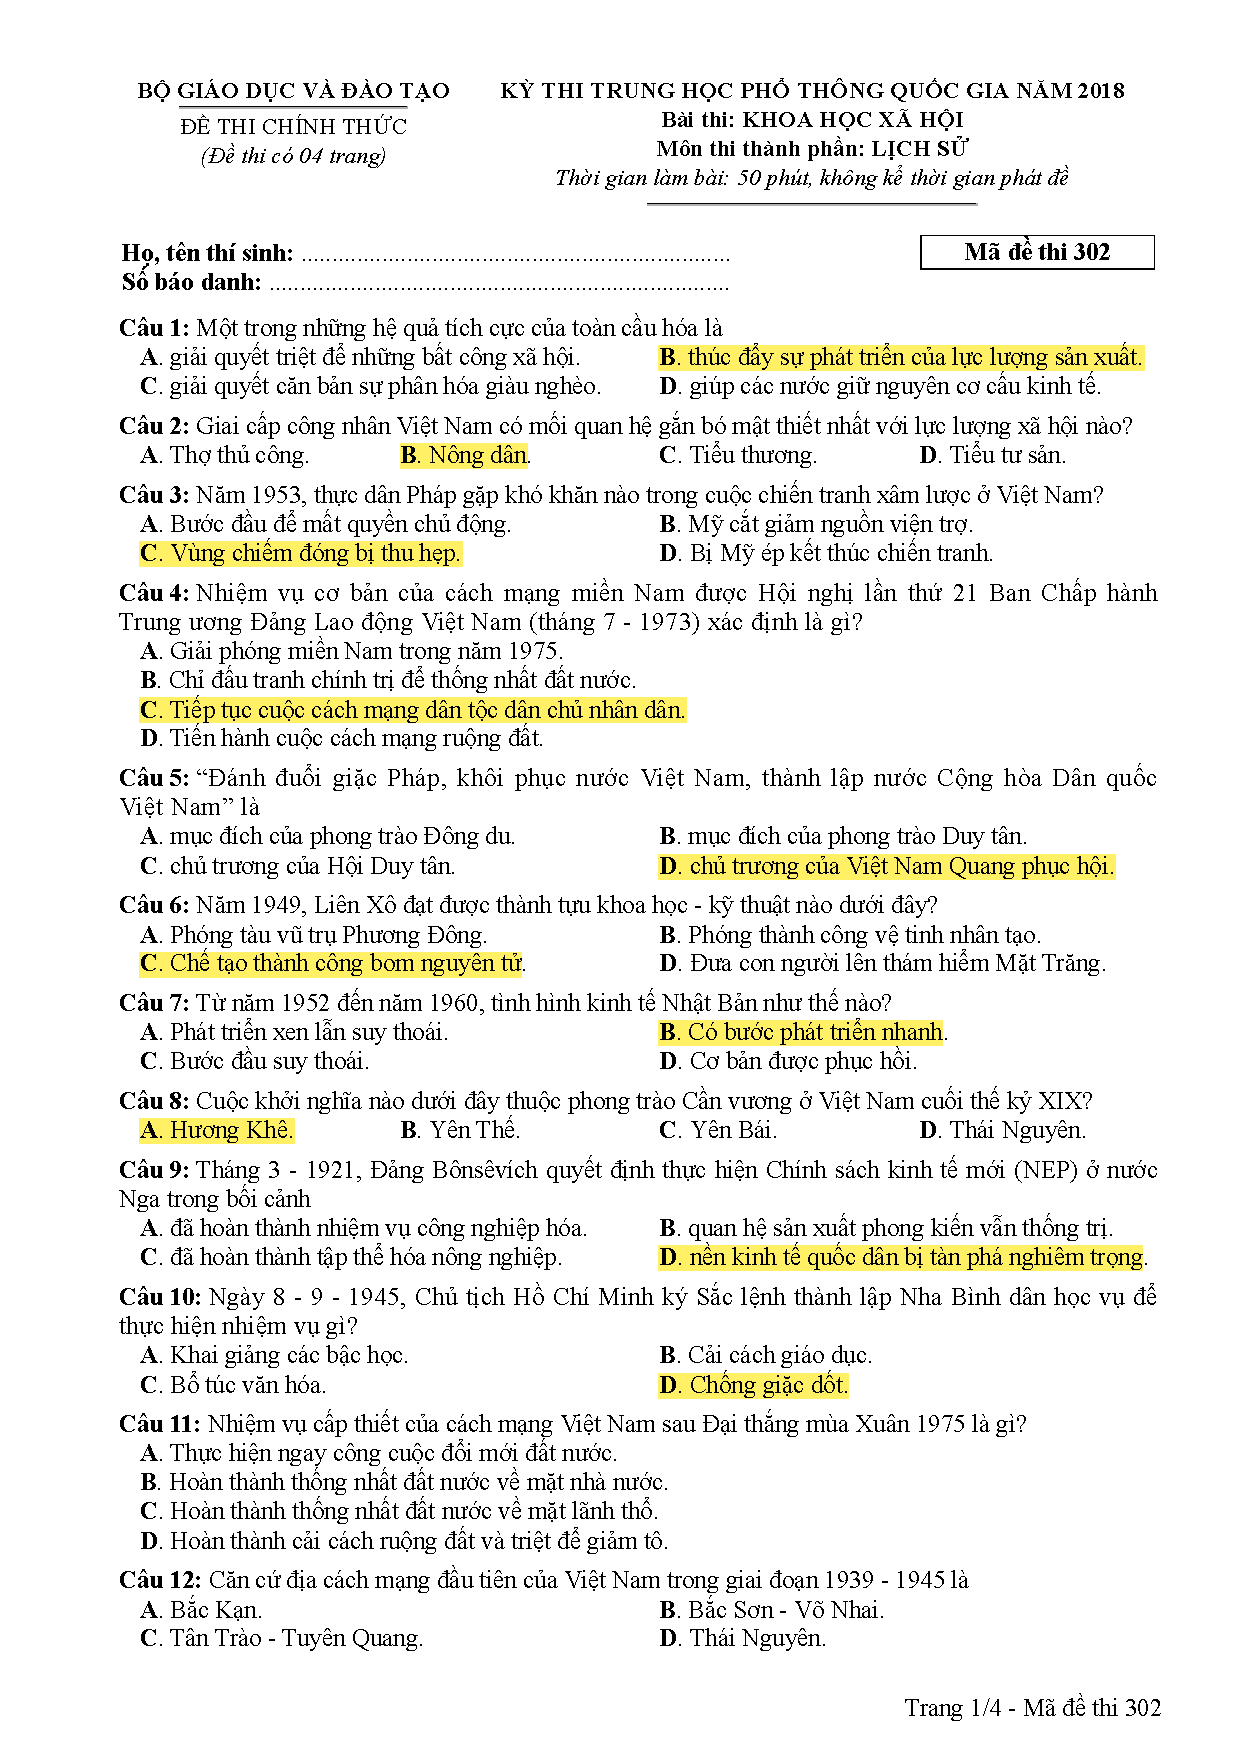
\includegraphics[width=1\textwidth, page=1]{Appendix/Fig/2018_302.pdf}
    \caption{Trang 1 đề thi THPT Lịch sử 2021}
\end{figure}

\begin{figure}[htbp]
    \centering
    \includegraphics[width=1\textwidth, page=2]{Appendix/Fig/2018_302.pdf}
    \caption{Trang 2 đề thi THPT Lịch sử 2021}
\end{figure}

\begin{figure}[htbp]
    \centering
    \includegraphics[width=1\textwidth, page=3]{Appendix/Fig/2018_302.pdf}
    \caption{Trang 3 đề thi THPT Lịch sử 2021}
\end{figure}

\begin{figure}[htbp]
    \centering
    \includegraphics[width=1\textwidth, page=4]{Appendix/Fig/2018_302.pdf}
    \caption{Trang 4 đề thi THPT Lịch sử 2021}
\end{figure}


\begin{table}[ht]
    \centering
    \caption{Câu trả lời của phương pháp đề xuất cho đề thi THPT Lịch sử 2018, mã đề 302. Với các câu in đậm là câu trả lời sai}
    \resizebox{\textwidth}{!}{
        \small
        \begin{tabular}{|>{\centering\arraybackslash}m{1.5cm}|*{10}{>{\centering\arraybackslash}m{1cm}|}}
            \hline
            \textbf{Câu}    & 1  & 2           & 3  & 4           & 5  & 6  & 7  & 8  & 9  & 10          \\ \hline
            \textbf{Đáp án} & B  & B           & C  & C           & D  & C  & B  & A  & D  & D           \\ \hline
            \textbf{Câu}    & 11 & 12          & 13 & 14          & 15 & 16 & 17 & 18 & 19 & 20          \\ \hline
            \textbf{Đáp án} & B  & B           & A  & C           & C  & C  & A  & B  & B  & B           \\ \hline
            \textbf{Câu}    & 21 & 22          & 23 & \textbf{24} & 25 & 26 & 27 & 28 & 29 & \textbf{30} \\ \hline
            \textbf{Đáp án} & A  & D           & D  & \textbf{D}  & B  & B  & A  & C  & A  & \textbf{C}  \\ \hline
            \textbf{Câu}    & 31 & \textbf{32} & 33 & 34          & 35 & 36 & 37 & 38 & 39 & 40          \\ \hline
            \textbf{Đáp án} & D  & \textbf{C}  & D  & A           & C  & A  & B  & C  & D  & C           \\ \hline
        \end{tabular}
    }
\end{table}



\end{document}
